\documentclass[11pt,a4paper]{report}
\usepackage[utf8]{inputenc}
\usepackage[T1]{fontenc}
\usepackage{lmodern}
\usepackage[french]{babel}
\usepackage[a4paper,margin=2.4cm]{geometry}
\usepackage{amsmath,amssymb}
\usepackage{graphicx}
\usepackage{booktabs}
\usepackage{array}
\usepackage{tabularx}
\usepackage{float}
\usepackage{caption}
\usepackage{xcolor}
\usepackage{enumitem}
\usepackage{fancyhdr}
\usepackage{titlesec}
\usepackage{tikz}
\usetikzlibrary{arrows.meta,positioning,calc,fit,backgrounds}
\usepackage{adjustbox}
\usepackage{newunicodechar}
\newunicodechar{Δ}{\ensuremath{\Delta}}
\newunicodechar{µ}{\ensuremath{\mu}}
\newunicodechar{≥}{\ensuremath{\geq}}
\newunicodechar{≤}{\ensuremath{\leq}}
\newunicodechar{×}{\ensuremath{\times}}
\newunicodechar{≈}{\ensuremath{\approx}}
\newunicodechar{→}{\ensuremath{\rightarrow}}
\newunicodechar{−}{\ensuremath{-}}
\usepackage[colorlinks=true,linkcolor=blue!50!black,citecolor=blue!50!black,urlcolor=blue!50!black]{hyperref}

% Figures produites par le notebook (../figures) ; logo INPT dans le dossier de la plateforme
\graphicspath{{../figures/}{../../}}
\definecolor{inptblue}{RGB}{0,114,188}
\definecolor{embb}{HTML}{2A78D6}
\definecolor{urllc}{HTML}{EB6834}
\definecolor{mmtc}{HTML}{1BAF7A}
\definecolor{muted}{HTML}{52514E}
\titleformat{\chapter}[hang]{\Large\bfseries\color{inptblue}}{\thechapter.}{0.6em}{}
\titlespacing*{\chapter}{0pt}{-10pt}{15pt}
\pagestyle{fancy}
\fancyhf{}
\fancyhead[L]{\small Projet SMARTICT -- Network slicing B5G et GNN}
\fancyhead[R]{\small INPT -- Filière Smart ICT}
\fancyfoot[C]{\thepage}
\setlength{\headheight}{14pt}
\captionsetup{font=small,labelfont=bf}
\renewcommand{\arraystretch}{1.15}
\setlength{\parskip}{0.4em}
\newcommand{\gnn}{\textsc{gnn}}
\newcommand{\R}{\mathbb{R}}

\begin{document}

\begin{titlepage}
\centering
\hfill\includegraphics[width=5cm]{INPT.png}\\[1.5cm]
{\large Institut National des Postes et Télécommunications}\\[0.3cm]
{\large Filière : Smart ICT}\\[2cm]
{\Huge\bfseries\color{inptblue} Projet SMARTICT}\\[0.6cm]
{\huge\bfseries AI-Based Dynamic Resource Allocation\\[0.2cm] for B5G Network Slicing}\\[0.8cm]
{\Large Prédire la QoS des slices avec un réseau de neurones sur graphe\\ et tester sa robustesse aux changements brusques du réseau}\\[2.5cm]
\begin{tabular}{rl}
\textbf{Réalisé par :} & El Mehdi LAZAAR\\[4pt]
 & EL KARFI Soufia\\[4pt]
 & ABOUBAKAR Sidiki\\[4pt]
 & Nizar BENSELLOUM\\[10pt]
\textbf{Encadrant :} & M. Hassan EL GHAZI
\end{tabular}
\vfill
\end{titlepage}

\begin{abstract}
\noindent Le \emph{network slicing} partage une infrastructure 5G/B5G entre des services aux exigences opposées (eMBB, URLLC, mMTC). L'opérateur doit réserver à chaque slice une part des ressources suffisante pour son contrat, et vérifier cette allocation quand le réseau change brusquement. À partir du dataset \emph{B5G Network Slicing} (Farreras et al., 2024 : 7\,127 simulations paquet, 1,58 million de flux, 162 topologies réelles), nous formulons le problème comme un \textbf{jumeau numérique}. Il s'agit de prédire, pour chaque flux, son délai (en log10) et son taux de pertes à partir de la topologie, du routage, des demandes et des poids WFQ réservés aux slices.

L'exploration révèle des pièges qui faussent silencieusement toute modélisation. 42\,\% des chemins du fichier de slices diffèrent du routage simulé, ce qui laisse 8\,\% des flux sans réservation sur leur port d'antenne. Le débit réel vaut 1,25 fois le débit nominal. 93\,\% des flux ont un jumeau aux entrées identiques. Nous les corrigeons ou les documentons avant toute modélisation.

Nous définissons un événement comme un écart brusque au régime habituel du réseau : identificateur de Hampel sur la charge du goulot de chaque flux, environ 14\,\% des flux. Nous comparons, sur des topologies jamais vues, une référence naïve, Ridge, Gradient Boosting, un MLP et un GNN hétérogène flux / files WFQ / liens inspiré de RouteNet.

Le GNN est le plus précis : MAE de 0,175 décade sur le délai (0,277 pour le Gradient Boosting) et de 0,045 sur les pertes (0,067). Surtout, il est le plus robuste pendant les événements : 0,271 contre 0,664. L'ablation montre que ce gain vient de deux sources : les interactions entre flux (sans rétroaction, l'erreur remonte à 0,240) et la représentation explicite des files WFQ par slice (sans elles, 0,428). Nous concluons qu'un GNN apporte une valeur ajoutée quand la QoS dépend de ressources partagées et d'effets en cascade, quand le graphe porte explicitement le levier d'allocation, et surtout quand le réseau sort de son régime habituel.
\end{abstract}


\tableofcontents
\listoffigures
\listoftables

%=====================================================================
\chapter*{Introduction générale}\addcontentsline{toc}{chapter}{Introduction générale}\markboth{Introduction générale}{}
%=====================================================================
Le \emph{network slicing} découpe une même infrastructure 5G/B5G en réseaux logiques, les \emph{slices}, adaptés chacun à un service. La slice \textbf{eMBB} privilégie le débit, la slice \textbf{URLLC} la latence et la fiabilité, la slice \textbf{mMTC} (ou mIoT) le nombre de terminaux. Ces slices partagent les mêmes antennes et les mêmes liens de transport. L'opérateur doit donc réserver à chacune une part des ressources suffisante pour son contrat de service (SLA), sans gaspiller la capacité. Quand le trafic change brusquement (pic de demande, nouvelle slice, réservation réduite), une allocation correcte peut devenir mauvaise.

Le guide du projet pose la question suivante : \emph{peut-on apprendre à partir des données une stratégie ou une prédiction utile pour la gestion des ressources des slices, et cette solution reste-t-elle fiable lors de changements brusques du réseau ?} Il demande de construire et de justifier notre propre démarche, puis de répondre à la question finale : \emph{dans quelles conditions une approche \gnn{} apporte-t-elle une valeur ajoutée pour la gestion dynamique des slices B5G ?}

Notre démarche :
\begin{enumerate}[nosep]
  \item situer le problème dans la littérature : network slicing, allocation des ressources, réseaux de neurones sur graphes et leurs applications aux réseaux (chapitre~\ref{chap:sota}) ;
  \item explorer le dataset \emph{B5G Network Slicing} (Farreras et al., 2024) : 7\,127 simulations paquet, 1,58 million de flux (chapitre~\ref{chap:data}) ;
  \item formuler le problème comme un \textbf{jumeau numérique} : prédire la QoS (délai, pertes) de chaque flux d'une slice à partir de la configuration du réseau et des réservations (chapitre~\ref{chap:pb}) ;
  \item construire des références sans graphe : modèle naïf, Ridge, Gradient Boosting, MLP (chapitre~\ref{chap:base}) ;
  \item définir les événements comme des écarts brusques au régime habituel du réseau (chapitre~\ref{chap:evt}) ;
  \item représenter chaque simulation par un graphe hétérogène flux / files WFQ / liens et entraîner un \gnn{} de type RouteNet (chapitre~\ref{chap:gnn}) ;
  \item comparer globalement, pendant les événements, par ablation et sous décalage de distribution (chapitre~\ref{chap:res}), puis discuter et conclure (chapitres~\ref{chap:disc} et~\ref{chap:concl}).
\end{enumerate}
Tout le code (extraction, features, modèles, évaluation) est dans le notebook du projet (\path{projet_B5G_slicing_GNN.ipynb}) et dans le dossier \texttt{code/}. L'annexe~\ref{chap:annexe} décrit comment reproduire les résultats ; un guide séparé (\path{Guide_du_code.pdf}) détaille le contenu de chaque fichier.

%=====================================================================
\chapter{État de l'art : network slicing et réseaux de neurones sur graphes}\label{chap:sota}
%=====================================================================
Ce chapitre pose les notions nécessaires au reste du rapport. La section~\ref{sec:sota-slicing} présente le network slicing et ses exigences. La section~\ref{sec:sota-alloc} décrit le problème d'allocation des ressources entre slices et les approches qui le traitent. La section~\ref{sec:sota-gnn} introduit les réseaux de neurones sur graphes (\gnn), et la section~\ref{sec:sota-gnnnet} leurs applications aux réseaux de communication. La section~\ref{sec:sota-position} situe notre travail par rapport à cet état de l'art et annonce la démarche des chapitres suivants.

%---------------------------------------------------------------------
\section{Le network slicing en 5G et au-delà}\label{sec:sota-slicing}
%---------------------------------------------------------------------
\subsection{Trois familles d'usages aux exigences opposées}
La recommandation ITU-R M.2083~\cite{itu2083} définit trois scénarios d'usage pour les réseaux IMT-2020 (5G) :
\begin{itemize}
  \item \textbf{eMBB} (\emph{enhanced Mobile Broadband}) : très haut débit pour la vidéo, la réalité virtuelle, l'accès fixe sans fil. Les objectifs sont de 20~Gbit/s en débit crête et de 100~Mbit/s en débit perçu par l'utilisateur ;
  \item \textbf{URLLC} (\emph{Ultra-Reliable Low-Latency Communications}) : contrôle industriel, véhicules, chirurgie à distance. Les objectifs sont une latence de 1~ms sur l'interface radio et une fiabilité de $1-10^{-5}$ pour un paquet de 32 octets~\cite{tr38913} ;
  \item \textbf{mMTC} (\emph{massive Machine-Type Communications}, appelée mIoT dans le dataset) : capteurs et objets connectés en très grand nombre, jusqu'à $10^6$ terminaux par km², avec un faible débit et une forte tolérance au délai.
\end{itemize}
Ces exigences sont contradictoires. Un réseau unique dimensionné pour la plus exigeante de chaque contrainte coûterait très cher ; un réseau dimensionné « en moyenne » ne satisferait personne. Le \emph{network slicing} répond à ce dilemme.

\subsection{Définition et normalisation}
Une \textbf{slice} est un réseau logique de bout en bout, isolé et doté de ses propres caractéristiques, construit sur une infrastructure physique partagée. Le concept a été popularisé par le livre blanc 5G de l'alliance NGMN~\cite{ngmn}, puis normalisé par le 3GPP. Dans l'architecture 5G (TS~23.501~\cite{ts23501}), chaque slice est identifiée par un S-NSSAI qui contient un type de service (\emph{Slice/Service Type}). Les valeurs normalisées 1, 2 et 3 désignent précisément eMBB, URLLC et MIoT : ce sont les trois types de slices du dataset étudié. La gestion du cycle de vie d'une slice (préparation, mise en service, exploitation, retrait) est décrite par la TS~28.530~\cite{ts28530}.

Le slicing repose sur deux technologies de « softwarisation »~\cite{afolabi,foukas} :
\begin{itemize}
  \item la \textbf{virtualisation des fonctions réseau} (NFV), qui exécute les fonctions du cœur de réseau sur des serveurs génériques ;
  \item les \textbf{réseaux définis par logiciel} (SDN), qui séparent le plan de contrôle du plan de données et permettent de programmer l'acheminement et l'ordonnancement.
\end{itemize}
Une slice traverse tous les domaines du réseau : l'accès radio, le réseau de transport et le cœur~\cite{rost}. Le dataset étudié couvre le \textbf{transport}, avec des antennes en entrée (chapitre~\ref{chap:data}).

\begin{figure}[H]
\centering
\begin{tikzpicture}[
  >=Stealth, font=\small,
  infra/.style={draw=muted, fill=black!4, rounded corners=3pt, minimum height=9mm, align=center},
  sl/.style={rounded corners=3pt, minimum height=7mm, align=center, text=white, font=\small\bfseries}]
\node[infra, minimum width=12.6cm] (phy) at (0,0) {Infrastructure physique partagée : antennes, liens de transport, serveurs du cœur};
\node[sl, fill=embb, minimum width=12.6cm] (e) at (0,1.15) {Slice eMBB : débit élevé (vidéo, réalité virtuelle)};
\node[sl, fill=urllc, minimum width=12.6cm] (u) at (0,2.05) {Slice URLLC : latence < 1 ms, fiabilité $1-10^{-5}$ (industrie, véhicules)};
\node[sl, fill=mmtc, minimum width=12.6cm] (m) at (0,2.95) {Slice mMTC : $10^6$ objets / km², faible débit (capteurs)};
\node[draw=inptblue, thick, rounded corners=3pt, fit=(e)(u)(m), inner sep=4pt, label={[font=\small, text=inptblue]right:\rotatebox{90}{SDN / NFV}}] {};
\node[font=\footnotesize, text=muted, align=center] at (0,-0.85) {Chaque slice reçoit une part réservée des ressources partagées : c'est le problème d'allocation.};
\end{tikzpicture}
\caption{Principe du network slicing : trois réseaux logiques isolés sur une même infrastructure.}
\label{fig:slicing}
\end{figure}

%---------------------------------------------------------------------
\section{L'allocation des ressources entre slices}\label{sec:sota-alloc}
%---------------------------------------------------------------------
\subsection{Le compromis isolation / mutualisation}
Allouer les ressources entre slices revient à arbitrer entre deux objectifs~\cite{foukas,afolabi}.
\begin{itemize}
  \item \textbf{L'isolation} : chaque slice doit tenir son SLA quoi que fassent les autres. Cela pousse à réserver largement (\emph{sur-provisionnement}), au prix de capacités inutilisées.
  \item \textbf{La mutualisation} (gain de multiplexage statistique) : les slices n'atteignent pas leur pic en même temps, donc on peut réserver moins que la somme des pics. Mais on risque alors le \emph{sous-provisionnement} quand la demande change brusquement.
\end{itemize}
L'allocation doit donc être \textbf{dynamique}, c'est-à-dire réajustée quand la charge évolue. Elle doit aussi être \textbf{vérifiée} : on veut savoir, avant de l'appliquer, si une nouvelle allocation respecte les SLA.

\subsection{Le mécanisme d'ordonnancement : WFQ}
Au niveau d'un port de sortie, le partage de capacité entre slices est réalisé par un ordonnanceur multi-files. Le modèle de référence est le \emph{Generalized Processor Sharing} (GPS) de Parekh et Gallager~\cite{gps}. Chaque file $i$ reçoit un poids $\phi_i$ et se voit garantir un débit d'au moins
\begin{equation}
g_i=\frac{\phi_i}{\sum_j \phi_j}\,C,
\end{equation}
où $C$ est la capacité du port. Le GPS est \emph{conservatif} : la capacité non utilisée par une file vide est redistribuée aux autres, au prorata de leurs poids. Le \emph{Weighted Fair Queuing} (WFQ)~\cite{wfq} est la version par paquets de GPS : il l'approche à un temps de transmission de paquet près. Dans le dataset étudié, chaque antenne applique WFQ avec une file par slice, et le poids de la file est la réservation de la slice. C'est le levier d'allocation que nous modélisons.

\subsection{Pourquoi la QoS est-elle difficile à prédire ?}
La théorie des files d'attente explique la non-linéarité du problème. Dans le modèle M/M/1 (arrivées poissonniennes de taux $\lambda$, service exponentiel de taux $\mu$), le temps moyen passé dans le système vaut~\cite{kleinrock}
\begin{equation}
T=\frac{1}{\mu-\lambda}=\frac{1}{\mu}\cdot\frac{1}{1-\rho},\qquad \rho=\frac{\lambda}{\mu}.
\end{equation}
Le délai \textbf{explose quand la charge $\rho$ approche 1}. Au-delà, avec une file de taille finie $B$, la file reste pleine : des paquets sont perdus et le délai sature autour de $B\,L/\mu$, le temps de vider $B$ paquets de taille $L$. La QoS change donc de \emph{régime} autour de $\rho=1$. Une petite variation de charge ou de réservation peut faire passer une slice d'un délai de quelques microsecondes à plusieurs millisecondes. C'est exactement le comportement observé dans le dataset (figure~\ref{fig:knee}, chapitre~\ref{chap:data}).

Dans un réseau, ces files sont de plus \textbf{couplées}. Les pertes subies par un flux sur un lien en amont réduisent la charge qu'il impose en aval. Les flux qui partagent un lien se ralentissent mutuellement. Les formules de file isolée ne s'appliquent plus : il faudrait résoudre un problème de point fixe à l'échelle du réseau entier.

\subsection{Trois familles d'approches}
\begin{table}[H]
\centering\small
\begin{tabularx}{\linewidth}{@{}>{\raggedright}p{2.6cm}>{\raggedright}X>{\raggedright\arraybackslash}X@{}}
\toprule
Approche & Principe & Limites\\
\midrule
Modèles analytiques & théorie des files d'attente (M/M/1, réseaux de Jackson) ; bornes de délai GPS~\cite{gps,kleinrock} & hypothèses fortes (trafic poissonnien, indépendance) ; mal adaptés aux régimes saturés et aux ordonnancements multi-files couplés\\
Simulation à événements discrets & simulateurs paquet comme OMNeT++~\cite{omnet}, qui reproduisent fidèlement le réseau & coûteuse : de quelques minutes à plusieurs heures par configuration dans le dataset étudié ; inutilisable dans une boucle d'optimisation\\
Apprentissage automatique & modèle appris sur des simulations ou des mesures : prévision de capacité par slice (DeepCog~\cite{deepcog}), prédiction de performance~\cite{routenet} & dépend des données ; risque de mal généraliser hors du régime d'entraînement\\
\bottomrule
\end{tabularx}
\caption{Approches pour évaluer une allocation de ressources entre slices.}
\label{tab:approaches}
\end{table}
Un modèle appris, rapide et fidèle, peut servir de \textbf{jumeau numérique du réseau}~\cite{digitaltwin} : une réplique logicielle qui évalue en millisecondes la conséquence d'une configuration avant de l'appliquer. Reste à choisir un modèle qui respecte la \emph{structure} du réseau. C'est la motivation des réseaux de neurones sur graphes.

%---------------------------------------------------------------------
\section{Les réseaux de neurones sur graphes}\label{sec:sota-gnn}
%---------------------------------------------------------------------
\subsection{Données relationnelles et invariance aux permutations}
Un graphe $G=(V,E)$ est formé de nœuds $V$ reliés par des arêtes $E$. Chaque nœud $v$ porte un vecteur d'attributs $x_v$. Les réseaux de neurones classiques traitent des vecteurs, des grilles (images) ou des séquences (texte). Un graphe n'a ni taille fixe ni ordre naturel de ses nœuds : un modèle sur graphe doit donc donner le même résultat quelle que soit la numérotation des nœuds (\emph{invariance} ou \emph{équivariance aux permutations}~\cite{battaglia}). Concaténer les attributs des nœuds dans un vecteur ne respecte pas cette propriété.

\subsection{Le passage de messages}
Presque tous les \gnn{} modernes suivent le cadre du \emph{message passing} formalisé par Gilmer et al.~\cite{mpnn}. À l'itération (ou couche) $t$, chaque nœud agrège les messages de ses voisins, puis met à jour son état :
\begin{equation}
m_v^{(t)}=\operatorname{AGG}\Big(\big\{\!\!\big\{\phi^{(t)}\big(h_v^{(t)},h_u^{(t)},e_{uv}\big):u\in\mathcal N(v)\big\}\!\!\big\}\Big),\qquad
h_v^{(t+1)}=\operatorname{UPD}^{(t)}\big(h_v^{(t)},m_v^{(t)}\big),
\label{eq:mp}
\end{equation}
avec $h_v^{(0)}=x_v$. L'agrégation AGG (somme, moyenne, maximum, attention) est insensible à l'ordre des voisins, ce qui garantit l'équivariance. Après $T$ itérations, l'état d'un nœud dépend de tout son voisinage à $T$ sauts : le \gnn{} apprend des \emph{interactions}, ce qu'un modèle à features indépendantes ne peut pas faire.

\begin{figure}[H]
\centering
\begin{tikzpicture}[>=Stealth, font=\small,
  n/.style={circle, draw=muted, minimum size=7mm, inner sep=0pt},
  c/.style={n, fill=embb!25}, o/.style={n, fill=black!6}]
\node[c] (v) at (0,0) {$v$};
\node[o] (a) at (-1.6,1.0) {$u_1$};
\node[o] (b) at (-1.8,-0.8) {$u_2$};
\node[o] (c) at (1.5,1.1) {$u_3$};
\node[o] (d) at (1.7,-0.9) {$u_4$};
\node[o] (e) at (-3.2,0.2) {$w$};
\draw (v)--(a) (v)--(b) (v)--(c) (v)--(d) (a)--(e) (b)--(e);
\draw[->, very thick, urllc] (a) -- (v); \draw[->, very thick, urllc] (b) -- (v);
\draw[->, very thick, urllc] (c) -- (v); \draw[->, very thick, urllc] (d) -- (v);
\node[font=\footnotesize, align=center] at (0,-1.8) {itération 1 : $v$ agrège $u_1,\dots,u_4$\\itération 2 : l'information de $w$ atteint $v$ via $u_1, u_2$};
\node[draw=muted, rounded corners=3pt, align=left, font=\footnotesize] at (6.0,0) {1. message $\phi(h_v,h_u,e_{uv})$ par voisin\\2. agrégation insensible à l'ordre\\3. mise à jour $h_v\leftarrow\operatorname{UPD}(h_v,m_v)$\\répété $T$ fois $\Rightarrow$ champ réceptif de $T$ sauts};
\end{tikzpicture}
\caption{Le passage de messages : chaque nœud agrège l'information de ses voisins, itération après itération.}
\label{fig:mp}
\end{figure}

\subsection{Les principales architectures}
\begin{table}[H]
\centering\small
\begin{tabularx}{\linewidth}{@{}>{\raggedright}p{2.6cm}>{\raggedright}X>{\raggedright\arraybackslash}X@{}}
\toprule
Architecture & Agrégation & Intérêt et limites\\
\midrule
GCN~\cite{gcn} & moyenne normalisée par les degrés, poids partagés & simple et efficace ; suppose un graphe homogène ; transductif dans sa forme d'origine\\
GraphSAGE~\cite{sage} & moyenne, max ou LSTM sur un échantillon de voisins & inductif : s'applique à des graphes jamais vus ; agrège un \emph{ensemble} sans ordre\\
GAT~\cite{gat} / GATv2~\cite{gatv2} & moyenne pondérée par une attention apprise & pondère les voisins selon leur pertinence ; GATv2 corrige l'attention « statique » de GAT\\
GIN~\cite{gin} & somme suivie d'un MLP & aussi expressif que le test de Weisfeiler-Lehman ; la somme distingue des multi-ensembles que la moyenne confond\\
Gated GNN~\cite{ggnn} & mise à jour par une cellule GRU~\cite{gru} & mémoire entre itérations, adaptée aux itérations nombreuses\\
R-GCN~\cite{rgcn}, HAN~\cite{han} & poids distincts par type de relation ou de nœud & graphes \emph{hétérogènes} (plusieurs types de nœuds et d'arêtes)\\
\bottomrule
\end{tabularx}
\caption{Principales familles de \gnn{} et leurs propriétés.}
\label{tab:gnnfamilies}
\end{table}
Le choix de l'agrégation n'est pas neutre. Xu et al.~\cite{gin} montrent que la somme conserve le \emph{nombre} de voisins, que la moyenne ne capture que leur \emph{distribution}, et que le maximum ne retient qu'un \emph{ensemble}. Quand le nombre de voisins varie de plusieurs ordres de grandeur, la somme peut aussi déstabiliser l'apprentissage. Le compromis courant consiste à moyenner et à donner le nombre de voisins comme attribut ; c'est notre choix au chapitre~\ref{chap:gnn}.

\subsection{Limites connues}
\begin{itemize}
  \item \textbf{Sur-lissage} (\emph{over-smoothing}) : en empilant de nombreuses couches de type GCN, les états des nœuds deviennent indiscernables~\cite{oversmoothing}.
  \item \textbf{Sur-compression} (\emph{over-squashing}) : l'information de voisinages lointains et nombreux est compressée dans un vecteur de taille fixe~\cite{oversquashing}. C'est problématique quand la cible dépend de dépendances à longue distance.
  \item \textbf{Généralisation hors distribution} : rien ne garantit qu'un \gnn{} entraîné sur de petits graphes reste précis sur de grands graphes, même si son architecture s'y applique sans modification~\cite{datasetshift}.
\end{itemize}
Ces limites guident notre protocole : nous évaluons sur des topologies inédites et sur des réseaux plus grands que ceux de l'entraînement.

%---------------------------------------------------------------------
\section{Les GNN pour les réseaux de communication}\label{sec:sota-gnnnet}
%---------------------------------------------------------------------
Un réseau de communication est naturellement un graphe. Les \gnn{} y sont appliqués à la modélisation de performance, au routage, à l'allocation de ressources radio et à la planification~\cite{suarez,jiang}.
\begin{itemize}
  \item \textbf{RouteNet}~\cite{routenet} prédit le délai, la gigue et les pertes de chaque flux à partir de la topologie, du routage et de la matrice de trafic. Son idée clé est de ne pas utiliser le graphe physique, mais un graphe \emph{biparti flux--liens}. Chaque flux est relié aux liens qu'il traverse. Un GRU parcourt le chemin de chaque flux, dans l'ordre, et les liens agrègent les états des flux qui les traversent ; ces deux étapes sont répétées $T$ fois. RouteNet généralise à des topologies non vues à l'entraînement.
  \item \textbf{RouteNet-Fermi}~\cite{routenetf} ajoute des nœuds « file » pour modéliser des ports à plusieurs files avec différents ordonnancements (FIFO, priorité stricte, WFQ, DRR) et différents modèles de trafic. C'est l'architecture la plus proche de notre problème, où le levier est un ordonnancement WFQ par slice.
  \item Pour la \textbf{gestion des ressources radio}, des \gnn{} apprennent directement des politiques d'allocation de puissance ou de bande~\cite{eisen,shen}. Ils exploitent l'équivariance aux permutations pour passer à l'échelle sur des réseaux de taille variable.
  \item Ces modèles sont présentés comme les briques de \textbf{jumeaux numériques de réseau}~\cite{digitaltwin}, capables d'évaluer des « et si ? » sans simulation.
\end{itemize}
Ces travaux visent surtout la précision moyenne sur des configurations semblables à l'entraînement. Deux questions restent peu étudiées : l'effet des \emph{réservations de slices} comme variable de décision, et la \emph{fiabilité} des prédictions quand le réseau sort brusquement de son régime habituel.

%---------------------------------------------------------------------
\section{Positionnement et démarche}\label{sec:sota-position}
%---------------------------------------------------------------------
Cet état de l'art conduit à trois constats qui structurent notre travail.
\begin{enumerate}
  \item \textbf{La QoS d'une slice est non linéaire et couplée} : régime de saturation autour de $\rho=1$, et interactions entre flux qui partagent des files et des liens. C'est l'argument théorique en faveur d'un modèle relationnel, et c'est une hypothèse que nous \emph{testons} plutôt que d'admettre (ablation du chapitre~\ref{chap:res}).
  \item \textbf{Un \gnn{} n'est pertinent que si son graphe porte le levier de décision.} En nous inspirant de RouteNet-Fermi, nous représentons explicitement les files WFQ par slice, où s'applique la réservation $\delta$.
  \item \textbf{La valeur d'un modèle se juge aussi hors régime habituel.} Nous définissons des événements (changements brusques de charge) et nous mesurons la robustesse de chaque modèle pendant ces événements. Nous comparons le \gnn{} à des références sans graphe exigeantes, et non à une seule baseline faible.
\end{enumerate}
La suite du rapport suit cette logique. Le chapitre~\ref{chap:data} explore le dataset et en corrige les défauts. Le chapitre~\ref{chap:pb} formule le problème comme un jumeau numérique et fixe un protocole sans fuite d'information. Les chapitres~\ref{chap:base} à~\ref{chap:gnn} construisent les références, les événements et le \gnn. Le chapitre~\ref{chap:res} compare tous les modèles, et les chapitres~\ref{chap:disc} et~\ref{chap:concl} répondent à la question finale du guide.


%=====================================================================
\chapter{Le dataset B5G Network Slicing}\label{chap:data}
%=====================================================================
\section{Origine et structure}
Le dataset est publié par Farreras, Paillissé, Fàbrega et Vilà (\emph{Data in Brief}, 2024, DOI 10.5281/zenodo.10610616)~\cite{farreras}. Il a été généré avec BNNetSimulator, un simulateur à événements discrets au niveau paquet construit sur OMNeT++~\cite{omnet}. Les topologies de transport sont réelles et proviennent de l'Internet Topology Zoo~\cite{topozoo}. Le simulateur y ajoute des antennes, des terminaux et des destinations pour trois types de slices, puis simule le réseau jusqu'au régime stationnaire. \textbf{Un échantillon est une simulation.}

\begin{table}[H]
\centering\small
\begin{tabularx}{\linewidth}{@{}lrX@{}}
\toprule
Fichier & Nombre & Contenu\\
\midrule
\texttt{graphs/graph\_n.txt} & 7\,985 & topologie GML : nœuds typés, ordonnancement, files, poids WFQ par port, capacités\\
\texttt{routings/routing\_n.txt} & 7\,985 & port de sortie à utiliser pour chaque destination\\
\texttt{slices/slices\_n.json} & 7\,985 & slices : type, $\delta$, flux (origine, antenne, destination, chemin, débit)\\
\texttt{results\_*.tar.gz} & 79 & 100 simulations chacune : délais, gigue, pertes par flux ; trafic ; utilisation des ports et des files ; stabilité\\
\bottomrule
\end{tabularx}
\caption{Fichiers du dataset (archive de 271~Mo, somme MD5 vérifiée).}
\end{table}

Chaque réseau simulé contient des nœuds \texttt{origin\_*} (terminaux d'une slice), des \textbf{antennes}, des nœuds de \textbf{transport} (\texttt{inner}) et des nœuds \texttt{destination\_*}. Un flux part d'un terminal, passe par une antenne, traverse le transport et atteint la destination de sa slice. Chaque port de sortie d'une antenne applique un ordonnancement \textbf{WFQ} (\emph{Weighted Fair Queuing}) avec \textbf{une file par slice} ; le poids de la file est la part de capacité réservée à la slice. C'est le levier de gestion des ressources étudié. Le transport est FIFO, avec une seule file de 32 paquets. La réservation suit $V_{res}=V_{min}+\delta(V_{max}-V_{min})$, avec $V_{min}$ et $V_{max}$ égaux à 90\,\% et 120\,\% du débit nominal de la slice et $\delta\in[0,1]$ tiré par slice~\cite{farreras}.

\section{Extraction}
Les fichiers de résultats sont des matrices $N\times N$ « à plat » de plusieurs mégaoctets par ligne. Nous avons écrit notre propre parseur (\texttt{code/extraction.py}) à partir de la documentation des formats. Le parseur fourni avec le dataset décode les fichiers JSON avec \texttt{jsonpickle}, qui peut exécuter du code arbitraire ; nous l'avons utilisé comme référence de format, sans l'exécuter. L'extraction, parallélisée sur 14 processus, produit quatre tables :
\begin{itemize}[nosep]
  \item \textbf{samples} : 7\,127 simulations (162 topologies, 16 à 765 nœuds) ;
  \item \textbf{flows} : 1\,576\,669 flux avec leur slice, leur demande, leur file WFQ, leur chemin et leur QoS mesurée ;
  \item \textbf{links} : 3\,538\,248 liens orientés avec leur capacité, leur utilisation et leurs pertes mesurées ;
  \item \textbf{queues} : 263\,287 files WFQ actives aux ports des antennes.
\end{itemize}
773 simulations dont le statut n'est pas \texttt{OK} (régime stationnaire non atteint) sont écartées, comme le fait le parseur officiel.

Trois pièges de format méritent d'être signalés : chacun fausse silencieusement toutes les features.
\begin{enumerate}[nosep]
  \item \textbf{Les chemins.} Le champ \texttt{path} des fichiers de slices ne correspond pas toujours au routage simulé : 42\,\% des flux, et 76\,\% des simulations comptent au moins un tel flux. Le trafic suit en réalité le fichier \texttt{routings/routing\_n.txt} (matrice nœud $\times$ destination $\to$ port de sortie), comme dans le parseur officiel. Nous reconstruisons chaque chemin à partir de ce routage. Avec les chemins des slices, un quart des files WFQ semblaient porter du trafic sans débit mesuré ; avec le routage, la charge offerte calculée et l'utilisation mesurée des liens concordent (corrélation 0,984 sur 1,68~million de liens).
  \item \textbf{Les poids WFQ} sont définis \emph{par port de sortie} (« ; » sépare les ports, « , » les files), alors que l'affectation ToS $\to$ file est définie par nœud.
  \item \textbf{L'identifiant de simulation} de \texttt{input\_files.txt} recommence à 0 dans chaque archive : l'identifiant global est le numéro du fichier \texttt{graph\_n.txt}.
\end{enumerate}
Nous n'avons détecté le premier piège qu'en confrontant nos features aux mesures de sortie. C'est la vérification la plus utile de tout le projet : un modèle entraîné sur ces chemins aurait appris sur des entrées fausses, sans aucun message d'erreur.

\section{Dictionnaire des variables}
\begin{table}[H]
\centering\scriptsize
\begin{tabularx}{\linewidth}{@{}>{\raggedright}p{2.6cm}>{\raggedright}p{3.6cm}>{\raggedright}p{1.7cm}>{\raggedright}p{1.5cm}X@{}}
\toprule
Variable & Signification & Type & Rôle & Justification\\
\midrule
\texttt{slice\_type} & type de slice du flux & catégorielle & demande & fixe débit, taille de paquet et SLA\\
$\delta$ (\texttt{delta}) & paramètre de réservation de la slice & réel $[0,1]$ & ressource & levier de l'opérateur\\
\texttt{bandwidth} & débit nominal du flux & bit/s & demande & 18 (eMBB), 3,5 (URLLC), 0,2 (mMTC) Mb/s\\
\texttt{avg\_pkts\_lambda} & paquets par seconde (Poisson) & réel & demande & intensité réelle du trafic\\
\texttt{pkt\_size} & taille moyenne réelle des paquets & bits & demande & moyenne des deux tailles de la loi binomiale\\
\texttt{offered} & débit offert $=\lambda\times$ taille & bit/s & demande & 1,25 $\times$ nominal (eMBB, mMTC)\\
\texttt{path} & chemin du flux & liste & contexte & ressources partagées\\
\texttt{wfq\_weight} & poids WFQ de la file du flux & \% & ressource & part réservée à la slice\\
\texttt{capacity} & capacité d'un lien & bit/s & ressource & 25 à 400 Mb/s\\
\texttt{schedulingPolicy} & ordonnancement & catégorielle & ressource & WFQ aux antennes, FIFO ailleurs\\
\texttt{queueSizes} & taille des files & paquets & ressource & constante (32) : non informative\\
\texttt{n\_nodes} & taille du réseau & entier & contexte & généralisation\\
\texttt{AvgDelay} & délai moyen par paquet du flux & s & QoS, cible & 10~µs à 1\,929~s : en log10\\
\texttt{p10}…\texttt{p90}, \texttt{Jitter} & percentiles et variance du délai & réels & QoS & redondants avec le délai\\
\texttt{PktsDrop/PktsGen} & taux de pertes du flux & $[0,1]$ & QoS, cible & seconde cible\\
\texttt{utilization}, \texttt{losses} & mesures des ports et des files & $[0,1]$ & QoS (sortie) & interdites en entrée (fuite)\\
\texttt{global\_*} & agrégats réseau mesurés & réels & QoS (sortie) & analyse seulement\\
\texttt{sim\_time}, \texttt{stability} & durée et convergence & réels & qualité & simulations non stables écartées\\
\bottomrule
\end{tabularx}
\caption{Dictionnaire des variables (livrable L1) : rôle potentiel et justification.}
\label{tab:dico}
\end{table}

\section{Qualité des données}
\begin{itemize}
  \item \textbf{Valeurs manquantes} : aucune dans les tables de flux, de files et de simulations. Dans la table des liens, seule la taille de paquet mesurée est indéfinie (\texttt{-nan}) sur les 1,85~million de liens sans trafic ; cette variable n'est pas utilisée.
  \item \textbf{Flux sans délai} : 9 flux ont un délai de $-1$, car tous leurs paquets sont perdus. Ils sont exclus de la cible délai.
  \item \textbf{Doublons} : il n'y a aucun doublon exact, mais \textbf{93,4\,\% des flux ont un « jumeau »} dans la même simulation, avec la même slice, la même antenne, la même file WFQ et le même chemin après l'antenne. Ces flux ne diffèrent que par leur terminal, relié à l'antenne par un lien d'accès dédié. Leur QoS mesurée est quasi identique : l'écart-type intra-groupe de log10(délai) vaut 0,01 décade. Nous les regroupons en 263\,287 \textbf{classes de flux} de poids $w$ (6 flux en moyenne). Une classe correspond exactement à une file WFQ active : « une slice à une antenne ». Toutes les pertes et métriques sont pondérées par $w$, donc exactement équivalentes à un calcul par flux, pour un coût divisé par 6.
  \item \textbf{Chemins incohérents} : voir ci-dessus ; corrigés en utilisant le routage simulé.
  \item \textbf{Anomalie de taille de paquet} : le champ « taille moyenne » de la chaîne de trafic vaut 6\,000~bits pour eMBB, alors que les deux tailles possibles valent 12\,000 et 18\,000~bits. Le débit mesuré (22,5~Mb/s pour 18~Mb/s nominaux) confirme que la taille réelle est la moyenne des deux, soit 15\,000~bits. Nous utilisons la taille réelle.
  \item \textbf{Sous-dimensionnement systématique} : la réservation est calculée sur le débit \emph{nominal} alors que le débit réel vaut 1,25 fois le nominal pour eMBB et mMTC. Résultat : 91\,\% des flux ont un débit offert supérieur à leur débit réservé. 51\,\% traversent au moins un lien de transport dont la charge offerte dépasse la capacité. Le dataset couvre donc surtout des régimes saturés. Ce n'est pas une erreur à corriger, mais une propriété à garder en tête.
  \item \textbf{Réservations hors chemin} : 8,1\,\% des flux traversent un port d'antenne où leur slice n'a \emph{aucune} réservation (poids WFQ résiduel de 0,001\,\%). Les réservations semblent avoir été placées selon le champ \texttt{path}, alors que le trafic suit le routage. Ces files sont quasi affamées : pertes médianes de 63\,\% et délais jusqu'à 1\,929~s. Nous conservons cet effet réel ; il produit la majorité des « surcharges » du chapitre~\ref{chap:evt}.
  \item \textbf{Valeurs extrêmes} : les délais atteignent 1\,929~s pour des files WFQ quasi affamées (poids de l'ordre de 0,05\,\%). La cible est donc prise en log10. Quelques poids WFQ légèrement négatifs (au plus $-0{,}03$\,\%, des résidus d'arrondi) sont ramenés à 0.
\end{itemize}

\section{Distributions et relations}
\begin{figure}[H]
\centering
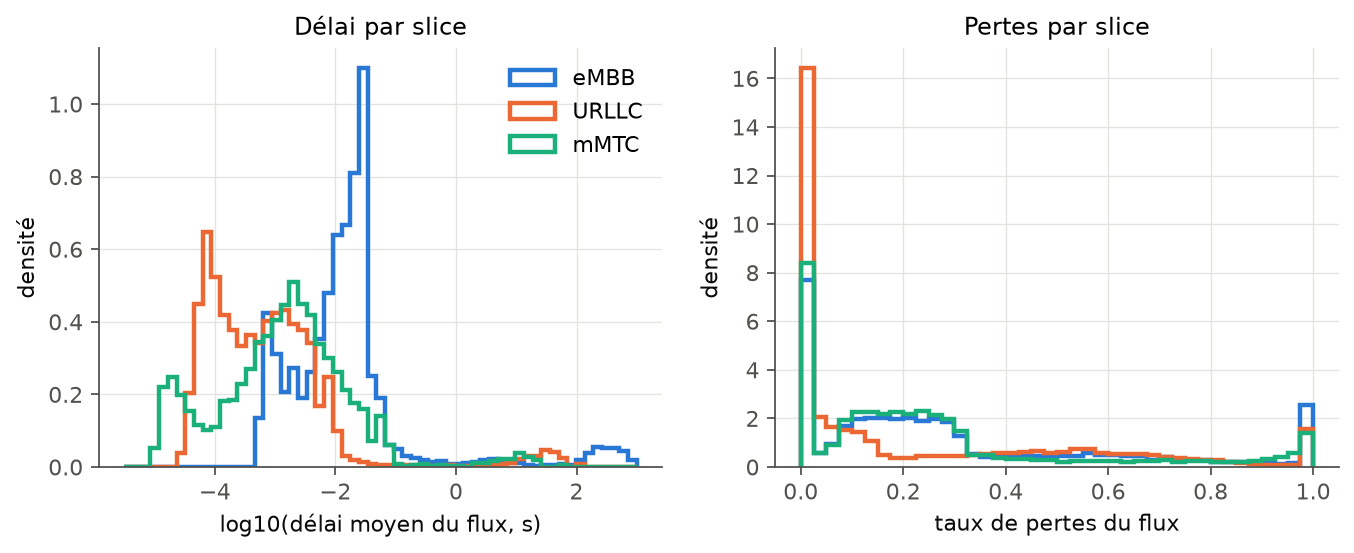
\includegraphics[width=\linewidth]{fig_targets.png}
\caption{Distribution du délai (log10) et du taux de pertes par type de slice (pondérée par flux).}
\label{fig:targets}
\end{figure}

Le délai couvre huit ordres de grandeur et sa distribution est \textbf{bimodale} (figure~\ref{fig:targets}). Un flux non congestionné ne subit que des temps de transmission, de 10~µs à 0,1~ms. Un flux congestionné attend derrière des files pleines, de la milliseconde à la seconde. Les délais médians valent 0,5~ms (URLLC), 1,6~ms (mMTC) et 13,8~ms (eMBB). Le taux de pertes médian atteint 7\,\% (URLLC), 19\,\% (mMTC) et 22\,\% (eMBB). On observe un pic à 0 (flux non congestionnés) et un pic à 1 (files affamées).

\begin{figure}[H]
\centering
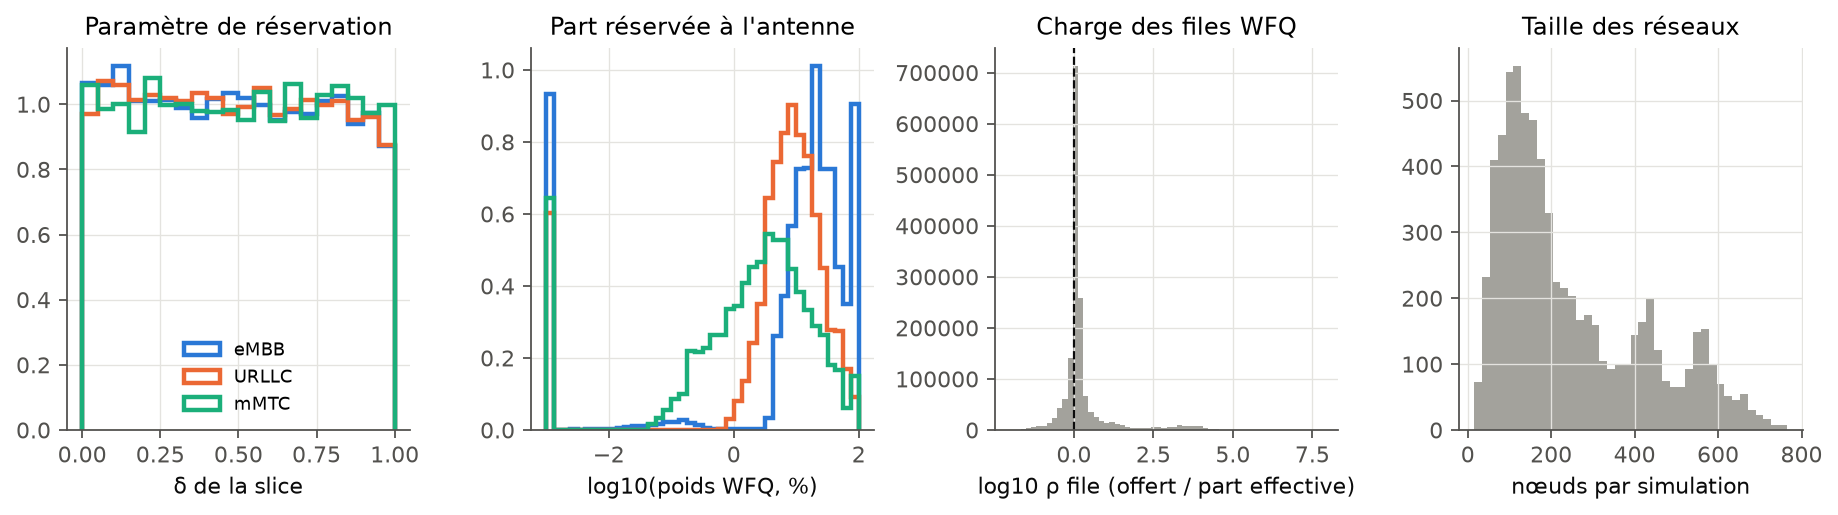
\includegraphics[width=\linewidth]{fig_inputs.png}
\caption{Entrées principales : $\delta$ (uniforme), poids WFQ par slice (échelle log), charge effective des files WFQ, taille des réseaux.}
\label{fig:inputs}
\end{figure}

Pour relier entrées et QoS, nous définissons pour chaque flux la \textbf{charge de son goulot}
\begin{equation}
b=\max\Big(\rho^{\text{file}}_{\text{eff}},\ \max_{\ell\in\text{chemin}}\rho_\ell\Big),\qquad
\rho_\ell=\frac{\sum_{f\ni\ell}\text{débit offert}_f}{C_\ell},\qquad
\rho^{\text{file}}_{\text{eff}}=\frac{\text{débit offert de la file}}{\frac{w_q}{\sum_{q'\text{ actives}}w_{q'}}\,C_{\text{port}}}.
\end{equation}
La part effective d'une file WFQ redistribue la capacité des files vides aux files actives, au prorata de leurs poids : c'est la propriété de conservation du GPS dont WFQ est la version par paquets~\cite{gps,wfq} (section~\ref{sec:sota-alloc}). $b$ ne dépend que des \emph{entrées} de la simulation : topologie, routage, demandes et poids.

\begin{figure}[H]
\centering
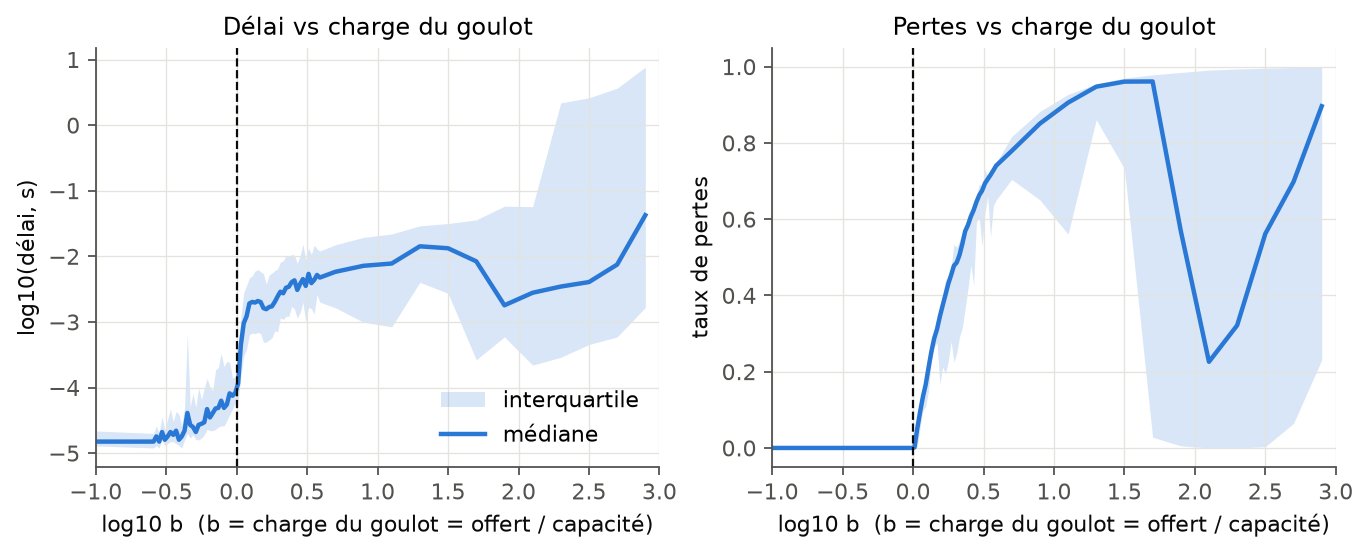
\includegraphics[width=0.9\linewidth]{fig_knee.png}
\caption{QoS médiane et interquartile en fonction de la charge du goulot $b$ : un coude net en $b=1$.}
\label{fig:knee}
\end{figure}

La figure~\ref{fig:knee} montre un \textbf{changement de régime en $b\approx1$}. En dessous, il n'y a pas de pertes et le délai reste de l'ordre de 10 à 100~µs. Au-dessus, les pertes croissent rapidement et le délai gagne deux décades. Comme $b$ couvre plus de dix ordres de grandeur (files affamées), l'axe est logarithmique. Les meilleures features isolées sont le délai de file pleine pour le délai ($|\rho_{\text{Spearman}}|=0{,}67$) et la charge effective de la file WFQ pour les pertes (0,73) (figure~\ref{fig:corr}). Aucune ne suffit pourtant : la QoS d'un flux dépend aussi des \emph{autres} flux qui partagent ses ressources, et des pertes qu'ils subissent en amont, qui allègent les liens en aval. C'est l'argument en faveur d'une représentation relationnelle, que l'ablation du chapitre~\ref{chap:res} met à l'épreuve.

\begin{figure}[H]
\centering
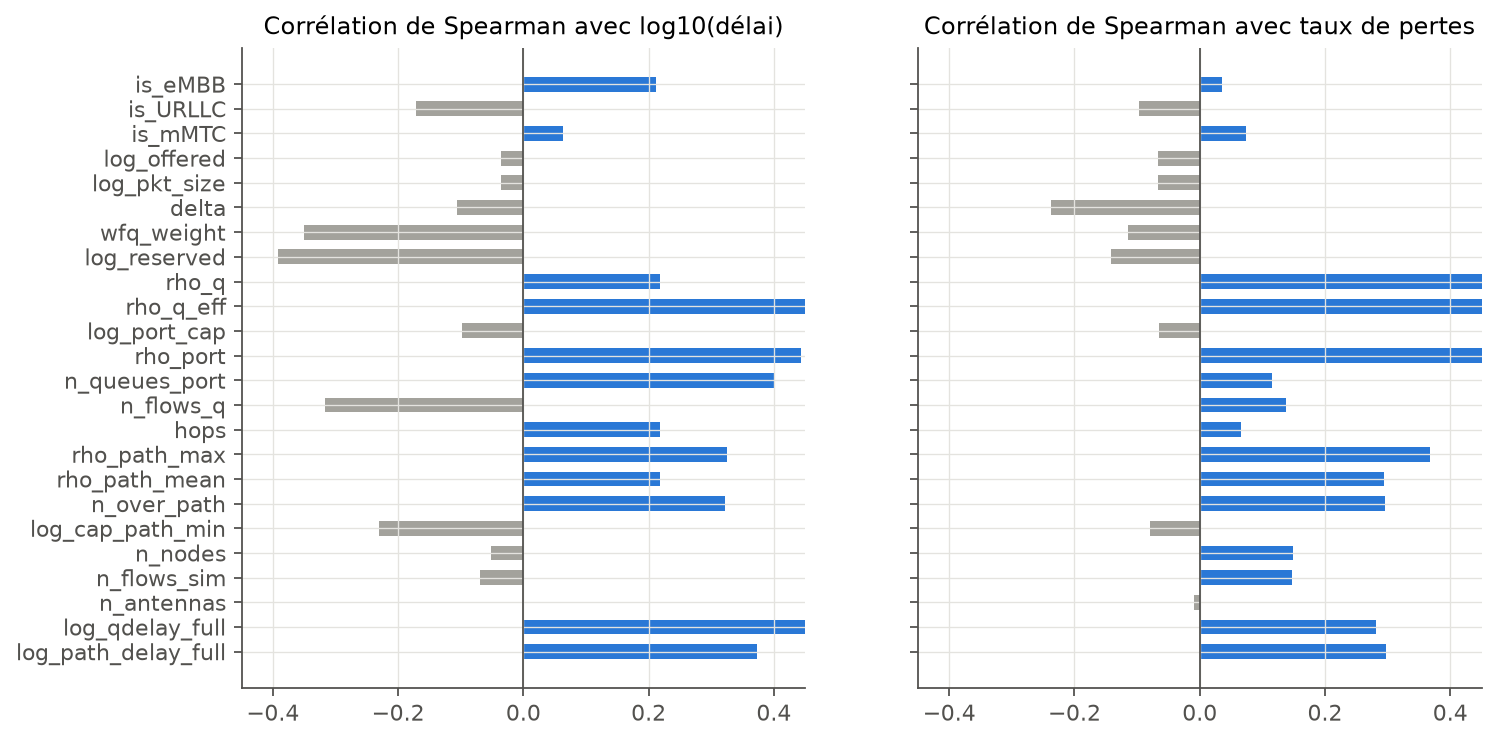
\includegraphics[width=0.85\linewidth]{fig_corr.png}
\caption{Corrélation de Spearman entre les 24 features et les deux cibles (300\,000 flux tirés au hasard).}
\label{fig:corr}
\end{figure}

\paragraph{Variables liées à la demande, aux ressources et à la QoS.} Demande : type de slice, débit offert, taille de paquet, nombre de flux. Ressources : $\delta$, poids et débit réservé WFQ, capacités, structure des files. QoS : délai, percentiles, gigue, pertes, et toutes les mesures d'utilisation. Ces dernières sont des sorties et ne sont jamais utilisées comme entrées.

%=====================================================================
\chapter{Formulation du problème et protocole}\label{chap:pb}
%=====================================================================
\section{Cible}
Pour chaque flux d'une slice, on prédit sa QoS en régime établi à partir de la configuration du réseau : topologie, routage, demandes de toutes les slices et réservations WFQ.
\begin{itemize}[nosep]
  \item $y_1=\log_{10}(\text{délai moyen})$, cible principale. Une MAE de 0,3 décade correspond à une erreur d'un facteur 2 environ. Le passage au logarithme est justifié de deux façons. D'une part, le délai couvre huit ordres de grandeur : en échelle linéaire, quelques files affamées (délais de plusieurs secondes) écraseraient toute la fonction de perte. D'autre part, l'erreur absolue sur le log est la moyenne du log du rapport prédit/réel, mesure recommandée pour les grandeurs strictement positives à forte dynamique, car elle pénalise symétriquement la sur- et la sous-estimation~\cite{tofallis}.
  \item $y_2=$ taux de pertes $\in[0,1]$, cible secondaire.
\end{itemize}

\section{Pourquoi cette cible est un problème de gestion des slices}
L'opérateur décide des réservations ($\delta$, donc des poids WFQ) et de l'admission des slices. Avant de déployer une configuration, il doit savoir si chaque slice respectera son SLA (tableau~\ref{tab:sla_def}). Une simulation paquet coûte entre quelques minutes et plusieurs heures : la colonne \texttt{sim\_time} atteint 15~h. Un prédicteur de QoS par flux répond en quelques millisecondes. Il sert de \textbf{jumeau numérique} pour (i) comparer des allocations candidates (« que se passe-t-il si je baisse $\delta$ de l'eMBB ? »), (ii) contrôler l'admission d'une nouvelle slice et (iii) détecter les slices qui vont violer leur SLA. C'est l'étape d'évaluation d'une boucle d'allocation dynamique, que l'optimisation des poids utilise ensuite.

Pourquoi pas une autre cible ? Prédire directement « la bonne allocation » est impossible : le dataset ne contient pas d'allocation optimale étiquetée, seulement des allocations aléatoires et leurs conséquences. Prédire l'utilisation des liens est moins utile : un SLA porte sur le délai et les pertes d'une slice, pas sur un lien.

\begin{table}[H]
\centering\small
\begin{tabular}{@{}lccc@{}}
\toprule
Slice & SLA délai & SLA pertes & Flux violant le SLA délai\\
\midrule
eMBB & 10~ms & 10\,\% & 59\,\%\\
URLLC & 0,5~ms & 0,001\,\% & 50\,\%\\
mMTC (mIoT) & 10~s & 1\,\% & 1\,\%\\
\bottomrule
\end{tabular}
\caption{Exigences des slices (Table~1 de~\cite{farreras}) et part des flux du dataset qui violent le SLA de délai.}
\label{tab:sla_def}
\end{table}

\section{Hypothèses}
\begin{description}[nosep]
  \item[H1] La QoS d'un flux dépend d'interactions entre flux : ressources partagées et pertes en amont. Un \gnn{} qui modélise ces interactions doit faire mieux que des modèles à features par flux.
  \item[H2] Les erreurs augmentent pendant les événements, quand la charge s'écarte du régime habituel du réseau.
  \item[H3] Les informations de réservation et de charge sont nécessaires : les retirer dégrade la prédiction.
\end{description}

\section{Protocole}
\begin{itemize}
  \item \textbf{Unité et métriques} : la classe de flux, de poids $w$. MAE et MSE sont pondérées par $w$ (donc par flux) et calculées sur les deux cibles.
  \item \textbf{Découpage par topologie} : chaque topologie est simulée environ 44 fois. Mélanger ses simulations entre entraînement et test permettrait de mémoriser la topologie. Les ensembles contiennent donc des topologies \textbf{disjointes} (tableau~\ref{tab:splits}). C'est la validation par blocs recommandée pour les données structurées en groupes : un découpage aléatoire des échantillons d'un même groupe surestime systématiquement la performance~\cite{roberts}.
  \item \textbf{Absence de fuite} : seules les entrées de la simulation servent de features. Normalisations et hyperparamètres sont fixés sur l'entraînement et la validation ; le test n'est évalué qu'une fois. Les mesures d'utilisation ou de pertes des liens seraient des prédicteurs très efficaces, mais elles ne sont connues qu'\emph{après} la simulation : les utiliser serait une fuite au sens de Kaufman et al.~\cite{kaufman}, et le modèle serait inutilisable pour évaluer une configuration nouvelle.
  \item \textbf{Décalage de distribution} : un second découpage (\texttt{shift}) entraîne sur les petits et moyens réseaux et teste sur les plus grands (quart supérieur des tailles de topologie, à partir de 212 nœuds).
\end{itemize}
\begin{table}[H]
\centering\small
\adjustbox{max width=\linewidth}{\begin{tabular}{llrrr}
\toprule
Découpage & Partie & Simulations & Topologies & Nœuds (médiane) \\
\midrule
topo & train & 5005 & 111 & 183 \\
topo & val & 1080 & 25 & 185 \\
topo & test & 1042 & 26 & 170 \\
shift & train & 4378 & 87 & 170 \\
shift & val & 935 & 22 & 161 \\
shift & test & 1814 & 53 & 244 \\
\bottomrule
\end{tabular}}
\caption{Découpages train / validation / test (topologies disjointes).}
\label{tab:splits}
\end{table}

%=====================================================================
\chapter{Baselines et modèles sans graphe}\label{chap:base}
%=====================================================================
Les modèles sans graphe utilisent 24 features par flux calculées à partir des entrées, en six familles :
\begin{itemize}[nosep]
  \item \emph{slice} : type, log débit offert, log taille de paquet ;
  \item \emph{réservation} : $\delta$, poids WFQ, log débit réservé, $\rho^{\text{file}}$ nominal et effectif ;
  \item \emph{port d'antenne} : capacité, charge offerte, nombre de files, nombre de flux de la file ;
  \item \emph{chemin} : nombre de sauts, charge maximale et moyenne des liens, nombre de liens surchargés, capacité minimale ;
  \item \emph{réseau} : nombre de nœuds, de flux et d'antennes ;
  \item \emph{physique} : deux délais issus d'un modèle fluide, décrits ci-dessous.
\end{itemize}

\paragraph{Features physiques.} Tous les flux servis par une même file WFQ d'antenne suivent le même chemin et ont la même QoS. Connaître la file explique donc toute la variance des cibles, alors que connaître seulement la simulation et le type de slice n'en explique que 49\,\% (délai) et 56\,\% (pertes). L'unité réellement prédite est « une slice à une antenne », c'est-à-dire le niveau où s'applique la réservation. Quand une file de $B=32$ paquets est saturée, un paquet attend environ le temps nécessaire pour la vider. Nous en tirons deux features :
\begin{align}
\texttt{log\_qdelay\_full}&=\log_{10}\frac{B\,L_{\text{slice}}}{r_{\text{eff}}},\qquad r_{\text{eff}}=\frac{w_q}{\sum_{\text{actives}}w}\,C_{\text{port}},\\
\texttt{log\_path\_delay\_full}&=\log_{10}\!\!\sum_{\ell\in\text{chemin},\ \rho_\ell>1}\!\!\frac{B\,\bar L_\ell}{C_\ell},
\end{align}
où $\bar L_\ell$ est la taille moyenne des paquets offerts au lien $\ell$. Elles injectent une connaissance du domaine (files pleines, partage WFQ) que les modèles n'ont pas à réapprendre.

Les features de chemin et de physique sont déjà des \emph{résumés du graphe construits à la main}, ce qui rend la comparaison avec le \gnn{} exigeante.

\begin{table}[H]
\centering\small
\begin{tabularx}{\linewidth}{@{}lX@{}}
\toprule
Modèle & Description\\
\midrule
Naïf & médiane pondérée de chaque cible par type de slice (apprise sur l'entraînement) : la référence minimale\\
Ridge & régression linéaire régularisée~\cite{ridge} sur les features standardisées ; $\alpha$ choisi sur la validation parmi $\{0{,}01;\dots;100\}$\\
Gradient Boosting & boosting de gradient~\cite{friedman} sur histogrammes (\texttt{HistGradientBoostingRegressor}, même principe que LightGBM~\cite{lightgbm}), 400 arbres ; taux d'apprentissage, nombre de feuilles et taille minimale des feuilles choisis sur la validation (grille de 8 configurations)\\
MLP & 2 couches cachées de 128 neurones, Adam~\cite{adam}, arrêt précoce sur la validation~\cite{prechelt}. C'est un \gnn{} sans graphe : il voit les mêmes features résumées\\
\bottomrule
\end{tabularx}
\caption{Modèles de référence (un modèle par cible pour Ridge et le Gradient Boosting, un modèle multi-sortie pour le MLP).}
\end{table}

Leurs résultats sont présentés avec ceux du \gnn{} au chapitre~\ref{chap:res}.

%=====================================================================
\chapter{Définition des événements}\label{chap:evt}
%=====================================================================
\section{Contrainte du dataset}
Les simulations sont des régimes stationnaires \textbf{indépendants} : il n'y a pas d'axe temporel, donc pas d'« avant » ni d'« après » une rupture. En revanche, chaque topologie est simulée environ 44 fois avec des slices, des placements d'antennes et des réservations différents. Ces simulations décrivent le \textbf{régime habituel} de ce réseau. Un changement brusque (pic de trafic, ajout d'une slice, réduction de $\delta$) place un flux dans un état éloigné de ce régime habituel. C'est cet écart que nous mesurons.

\section{Mesure de changement et règle}
La variable d'état est la charge du goulot $b$ (équation du chapitre~\ref{chap:data}). Ce choix a deux raisons : elle pilote le changement de régime de la QoS (figure~\ref{fig:knee}), et elle ne dépend que des entrées, donc l'opérateur peut l'observer avant toute mesure de QoS. Comme $b$ couvre plus de dix ordres de grandeur, l'écart est mesuré sur $\log_{10}b$, c'est-à-dire de façon \textbf{multiplicative} (« deux fois plus chargé que d'habitude »). Pour chaque flux, l'écart robuste au régime habituel vaut
\begin{equation}
z=\frac{\log_{10}b-\text{médiane}_{\tau,s}(\log_{10}b)}{1{,}4826\cdot\operatorname{MAD}_{\tau,s}(\log_{10}b)},
\end{equation}
où la médiane et l'écart absolu médian (MAD) sont calculés sur tous les flux de la même topologie $\tau$ et du même type de slice $s$. Le facteur 1,4826 rend le MAD comparable à un écart-type~\cite{mad} ; un plancher de 0,02 décade évite les divisions par une dispersion nulle.

\textbf{Règle} : le flux est un événement si $|z|\ge3$.
\begin{itemize}[nosep]
  \item \textbf{surcharge} ($z\ge3$) : le goulot est beaucoup plus chargé que d'habitude, typiquement une slice dont la réservation est devenue très inférieure à sa demande ;
  \item \textbf{délestage} ($z\le-3$) : le goulot est beaucoup moins chargé que d'habitude, au point de repasser sous la saturation.
\end{itemize}

\paragraph{Justification du seuil.}
\begin{enumerate}[nosep]
  \item $|z|\ge3$ est l'\textbf{identificateur de Hampel}~\cite{hampel}, règle robuste standard de détection de valeurs aberrantes : environ 0,3\,\% des valeurs pour une loi normale. Leys et al.~\cite{leys} recommandent explicitement la médiane et le MAD plutôt que la moyenne et l'écart-type, et un seuil de 3 comme choix « très conservateur ». Médiane et MAD résistent aux valeurs extrêmes, contrairement à la moyenne et à l'écart-type. Les queues de $\log_{10}b$ sont lourdes : avec $|z|\ge2$, 19\,\% des flux seraient des « événements », ce qui n'est plus un changement exceptionnel.
  \item Le seuil isole 13,6\,\% des flux (10,6\,\% de surcharges, 2,9\,\% de délestages), assez pour une évaluation stable (29\,851 flux en test).
  \item Les événements coïncident avec un changement de régime de la QoS (tableau~\ref{tab:events}) : 100\,\% des flux en surcharge ont $b>1$ (pertes médianes de 85\,\%), et 99,3\,\% des flux en délestage ont $b<1$ (pertes nulles, délai médian de 25~µs).
\end{enumerate}
Nous avons écarté une définition au niveau de la simulation (écart de la charge totale du réseau), car la QoS se joue au niveau des files d'antenne : deux flux d'une même simulation peuvent être l'un saturé, l'autre non. Nous avons aussi écarté une définition à partir de la QoS mesurée : elle évaluerait les modèles sur un sous-ensemble choisi d'après la cible elle-même. Le masque sert \textbf{uniquement à l'évaluation} et n'est jamais une feature.

\begin{table}[H]
\centering\small
\adjustbox{max width=\linewidth}{\begin{tabular}{lrrrrrr}
\toprule
Type & Flux & $b$ médian & part $b>1$ & log10 délai méd. & pertes méd. & Part \\
\midrule
délestage & 46429 & 0{,}387 & 0{,}007 & -4{,}602 & 0{,}000 & 0{,}029 \\
normal & 1362347 & 1{,}263 & 0{,}858 & -2{,}915 & 0{,}166 & 0{,}864 \\
surcharge & 167893 & 148{,}320 & 1{,}000 & -1{,}918 & 0{,}854 & 0{,}106 \\
\bottomrule
\end{tabular}}
\caption{Répartition des flux par type d'événement et QoS médiane associée.}
\label{tab:events}
\end{table}

\begin{figure}[H]
\centering
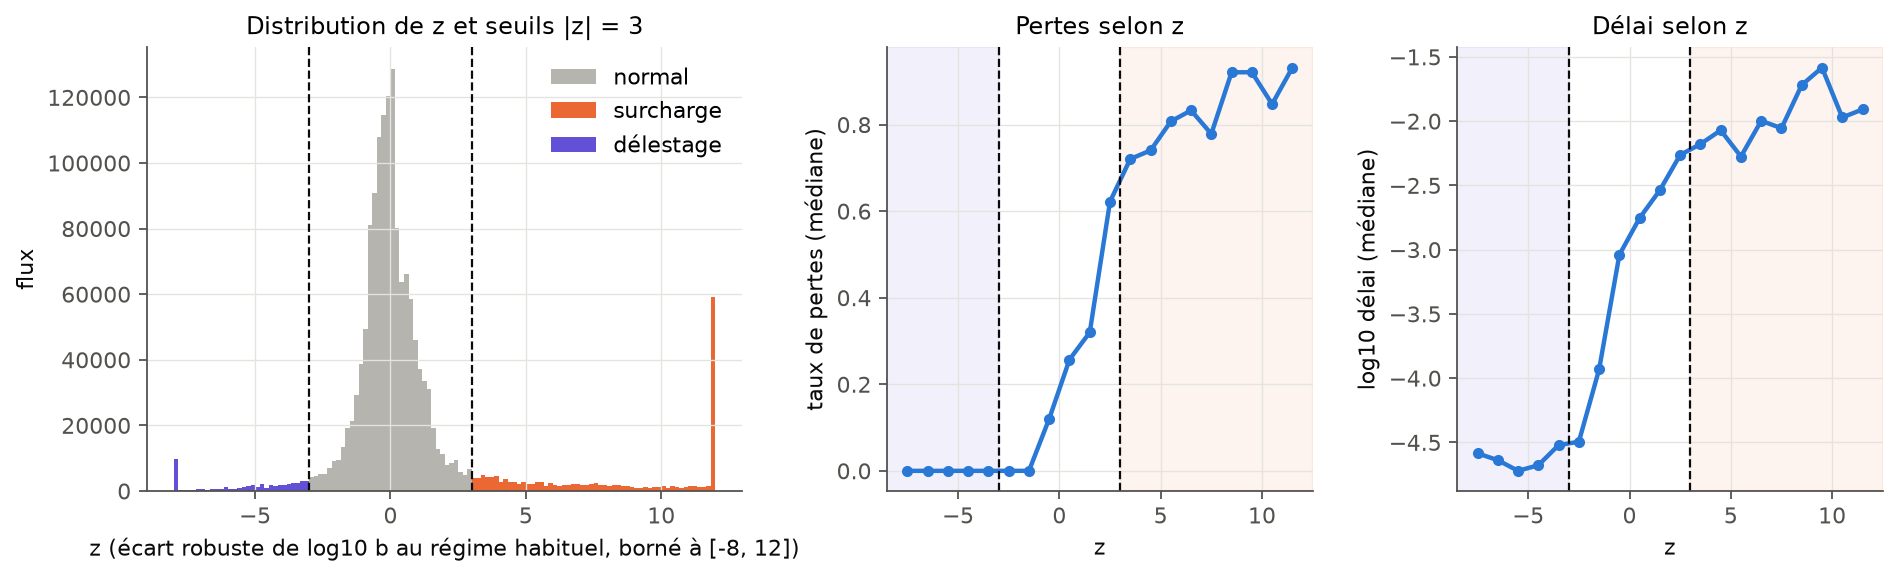
\includegraphics[width=\linewidth]{fig_events_z.png}
\caption{Distribution de $z$ avec les seuils $\pm3$, et QoS médiane en fonction de $z$.}
\label{fig:events_z}
\end{figure}

\section{Vérification visuelle}
\begin{figure}[H]
\centering
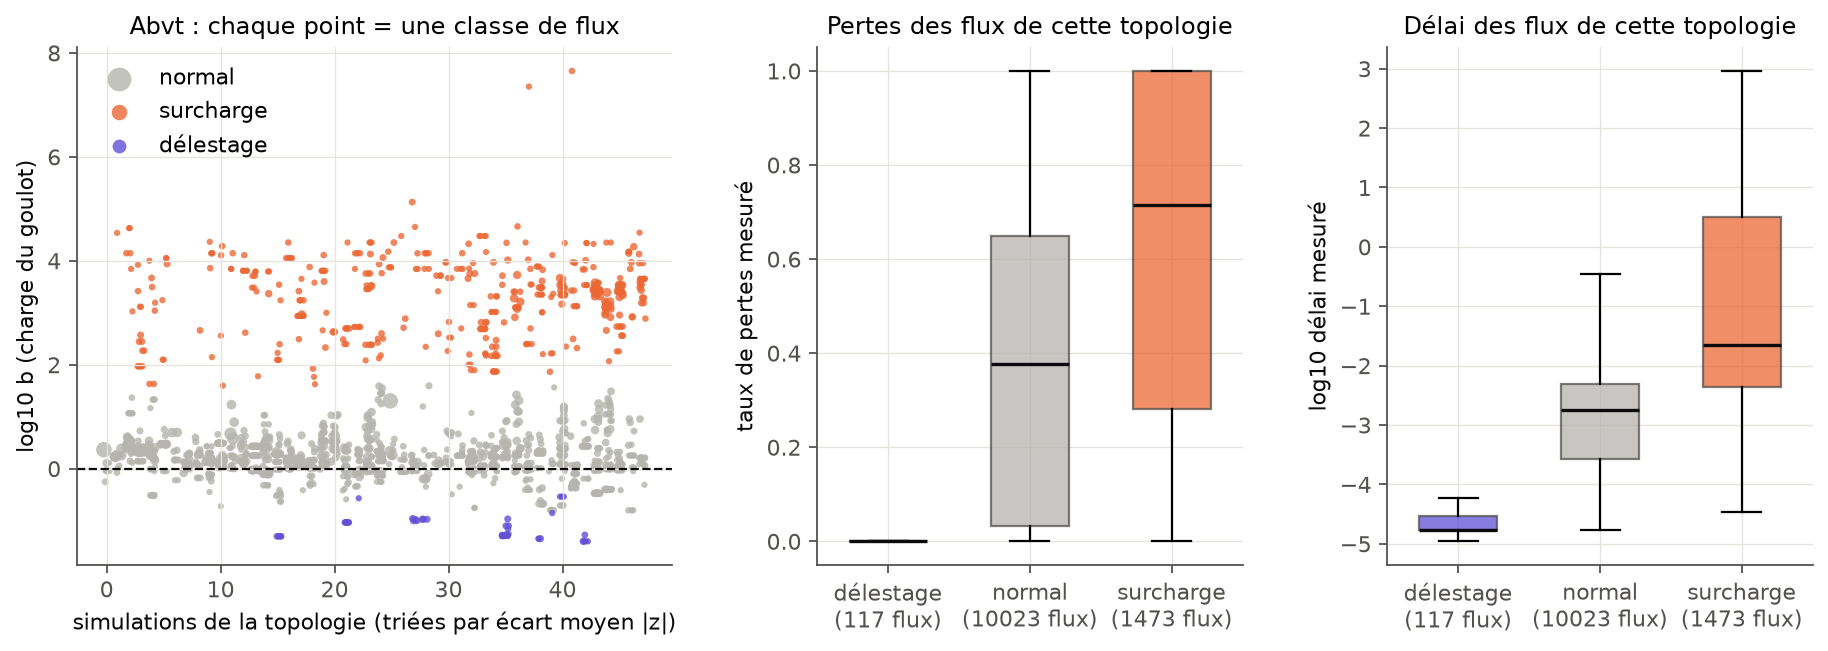
\includegraphics[width=\linewidth]{fig_events_topo.png}
\caption{Vérification sur une topologie. À gauche : charge du goulot de chaque classe de flux, simulation par simulation. Au centre et à droite : QoS mesurée des flux selon leur étiquette.}
\label{fig:events_topo}
\end{figure}
Sur une topologie simulée de nombreuses fois (figure~\ref{fig:events_topo}), les flux étiquetés sortent bien de la bande habituelle de $b$. Leur QoS mesurée diffère nettement : les flux en surcharge perdent plus de paquets et attendent plus longtemps. Les flux en délestage n'ont presque pas de pertes et un délai bien plus court. Le masque, construit sans regarder la QoS, isole donc des changements de régime réels.

%=====================================================================
\chapter{Représentation graphe et GNN}\label{chap:gnn}
%=====================================================================
\section{Le graphe}
Chaque simulation devient un \textbf{graphe hétérogène} à trois types de nœuds (tableau~\ref{tab:graph}).

\begin{table}[H]
\centering\small
\begin{tabularx}{\linewidth}{@{}lrX@{}}
\toprule
Nœuds & Nombre moyen & Attributs\\
\midrule
flux (classe de flux) & 37 & type de slice (one-hot), log débit offert, log taille de paquet, $\delta$, nombre de sauts\\
file WFQ (slice $\times$ port d'antenne) & 37 & poids WFQ, log débit réservé, $\rho^{\text{file}}$ nominal et effectif, log nombre de flux, log délai de file pleine\\
lien (traversé par un flux) & 15 & log capacité, charge offerte $\rho$, log nombre de flux, port d'antenne (0/1), log nombre de files, WFQ (0/1), log délai de file pleine\\
\midrule
\multicolumn{3}{@{}l}{Arêtes : flux $\to$ liens \textbf{ordonnées} (le chemin) ; flux $\to$ sa file WFQ ; file $\to$ le port (lien) de son antenne}\\
\bottomrule
\end{tabularx}
\caption{Graphe d'une simulation (moyennes sur les 7\,127 graphes ; 161 arêtes flux--lien en moyenne, chemins de 2 à 32 liens).}
\label{tab:graph}
\end{table}

\begin{figure}[H]
\centering
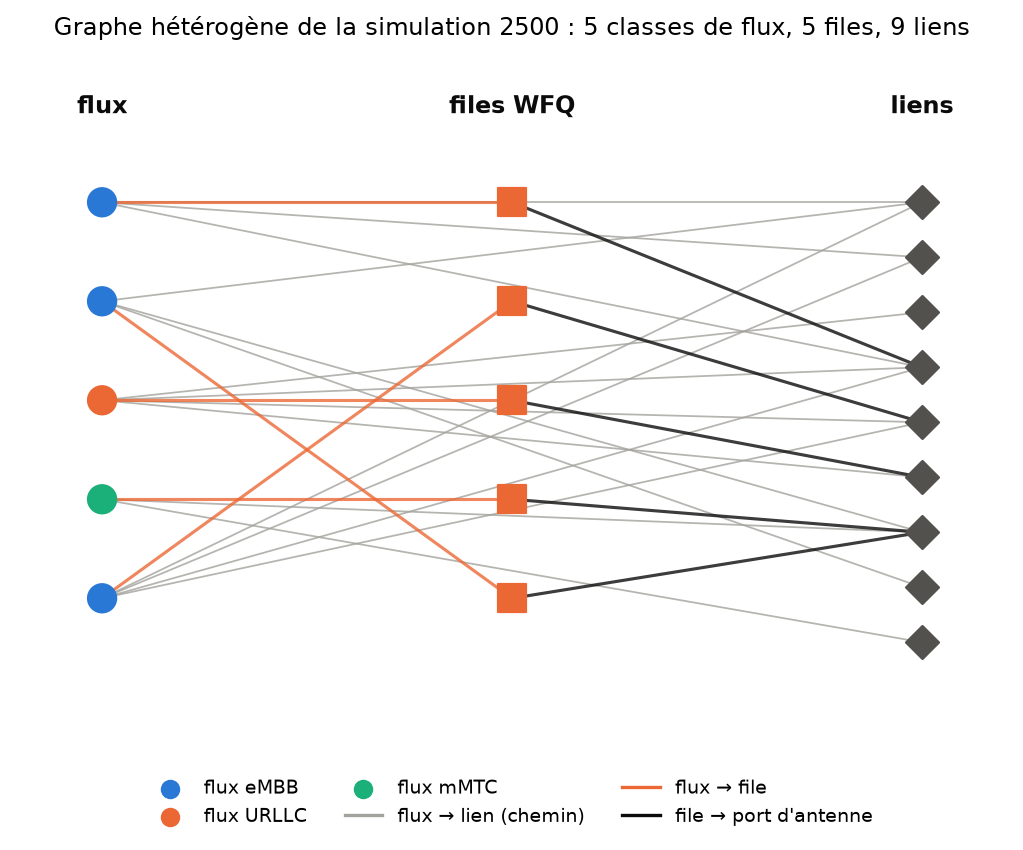
\includegraphics[width=0.72\linewidth]{fig_graph.png}
\caption{Graphe hétérogène d'une petite simulation : classes de flux (couleur = slice), files WFQ et liens.}
\label{fig:graph}
\end{figure}

\paragraph{Pourquoi des nœuds « flux » et « lien » plutôt que la topologie physique ?} On prédit la QoS d'un \emph{flux}. Elle dépend des ressources qu'il traverse et des autres flux qui les partagent. Le graphe physique (routeurs et câbles) ne contient pas l'information de routage. Le graphe biparti flux--liens, idée de RouteNet~\cite{routenet}, encode directement « qui partage quoi ».

\paragraph{Pourquoi des nœuds « file » ?} C'est à la file WFQ que s'applique la \textbf{réservation de slice}. Plusieurs slices partagent le port d'une antenne selon leurs poids : la file porte la part réservée, le lien la capacité totale.

\paragraph{Homogène ou hétérogène ?} Hétérogène : trois types de nœuds aux attributs différents, chacun avec ses propres fonctions de message et de mise à jour, comme dans les \gnn{} relationnels et hétérogènes~\cite{rgcn,han}. Partager les mêmes poids entre un flux et un lien n'aurait pas de sens physique.

\paragraph{Pourquoi plus informatif qu'un vecteur ?} Le vecteur de features résume le chemin par quelques statistiques (charge maximale et moyenne). Il ignore \emph{qui} partage chaque lien et \emph{combien de trafic arrive réellement} après les pertes en amont. Or le délai d'un flux dépend de l'état des autres flux, qui dépend lui-même du sien. C'est un problème de point fixe, que le passage de messages approche par itérations.

\section{Architecture}
Le modèle \texttt{SliceGNN} (\texttt{code/gnn.py}) s'inspire de RouteNet~\cite{routenet,routenetf}. Les états cachés ont la dimension $d=64$ ; trois MLP encodent les attributs des flux ($h_f$), des files ($h_q$) et des liens ($h_\ell$). On répète ensuite $T=4$ fois :
\begin{enumerate}
  \item \textbf{Flux $\leftarrow$ liens et file.} Comme dans RouteNet et les Gated GNN~\cite{routenet,ggnn}, chaque flux parcourt son chemin $(\ell_0,\dots,\ell_{K-1})$ avec un GRU initialisé par $h_f$ :
  \begin{equation}
  o_{f,k},\ s_{f,k}=\mathrm{GRU}\big([h_{\ell_k}\,;\,h_{q(f)}\,\mathbf{1}_{k=0}],\ s_{f,k-1}\big),\qquad s_{f,-1}=h_f,\qquad h_f\leftarrow s_{f,K-1}.
  \end{equation}
  Le premier lien $\ell_0$ est le port WFQ de l'antenne, où le flux lit aussi l'état de sa file. La sortie $o_{f,k}$ décrit le flux \emph{tel qu'il arrive} sur le lien $\ell_k$.
  \item \textbf{Liens $\leftarrow$ flux.} $m_\ell=\sum_{(f,k):\ell_k=\ell}w_f\,o_{f,k}\big/\sum w_f$ (moyenne pondérée par la multiplicité), puis $h_\ell\leftarrow\mathrm{GRUCell}(m_\ell,h_\ell)$.
  \item \textbf{Files $\leftarrow$ flux.} La même agrégation porte sur les flux servis par la file, à leur premier saut, puis $h_q\leftarrow\mathrm{GRUCell}(m_q,h_q)$.
\end{enumerate}
En sortie, un MLP ($64\to64\to32\to2$) appliqué à $h_f$ donne les deux cibles standardisées. La perte est la MSE pondérée par $w$, somme des deux cibles.

\begin{figure}[H]
\centering
\begin{tikzpicture}[
  box/.style={draw,rounded corners=2pt,minimum height=8mm,align=center,font=\small},
  fl/.style={box,fill=embb!15}, qu/.style={box,fill=urllc!18}, li/.style={box,fill=black!8},
  >=Stealth, node distance=6mm]
\node[fl] (xf) {attributs\\flux $x_f$};
\node[qu, below=of xf] (xq) {attributs\\files $x_q$};
\node[li, below=of xq] (xl) {attributs\\liens $x_\ell$};
\node[fl, right=12mm of xf] (hf) {$h_f$};
\node[qu, right=12mm of xq] (hq) {$h_q$};
\node[li, right=12mm of xl] (hl) {$h_\ell$};
\draw[->] (xf) -- node[above,font=\scriptsize]{MLP} (hf);
\draw[->] (xq) -- node[above,font=\scriptsize]{MLP} (hq);
\draw[->] (xl) -- node[above,font=\scriptsize]{MLP} (hl);
\node[box, right=18mm of hq, text width=4.6cm, inner sep=6pt, align=left, fill=white, font=\scriptsize] (mp)
  {{\small\textbf{passage de messages} $\times\,T=4$}\par\smallskip\raggedright
   1. GRU le long du chemin (le flux lit liens et file)\\
   2. liens $\leftarrow$ moyenne pondérée ($w$) des flux\\
   3. files $\leftarrow$ moyenne pondérée ($w$) des flux};
\draw[->] (hf) -- (mp.west |- hf);
\draw[->] (hq) -- (mp.west);
\draw[->] (hl) -- (mp.west |- hl);
\node[fl, right=14mm of mp] (out) {MLP\\$\to$ [log10 délai,\\pertes]};
\draw[->] (mp) -- node[above,font=\scriptsize]{$h_f$} (out);
\end{tikzpicture}
\caption{Architecture de SliceGNN.}
\label{fig:archi}
\end{figure}

\paragraph{Choix de l'architecture.} Nous ne l'avons pas choisie pour sa popularité, mais à partir des propriétés du graphe :
\begin{itemize}[nosep]
  \item le graphe est \textbf{hétérogène} et biparti, alors qu'un GCN homogène suppose des voisins de même nature ;
  \item l'information circule \textbf{le long de chemins ordonnés} : un flux qui perd des paquets en amont charge moins les liens en aval. Le GRU sur le chemin modélise cet ordre ; l'agrégation par ensemble de GraphSAGE ou de GAT l'ignore ;
  \item les dépendances sont \textbf{circulaires} (flux $\leftrightarrow$ liens) et longues : des itérations avec mémoire approchent ce point fixe mieux que quelques couches empilées ;
  \item le \textbf{nombre de voisins varie} fortement (de 1 à plusieurs centaines de flux par lien) : une moyenne pondérée reste stable, là où une somme exploserait. La moyenne perd l'information de cardinalité~\cite{gin} ; nous la réinjectons sous forme d'attribut (log du nombre de flux du lien et de la file).
\end{itemize}

\begin{table}[H]
\centering\small
\begin{tabular}{@{}ll@{}}
\toprule
Hyperparamètre & Valeur\\
\midrule
dimension cachée $d$ & 64\\
itérations $T$ & 4\\
optimiseur & Adam, taux $10^{-3}$, décroissance de poids $10^{-5}$\\
lot & 16 simulations\\
époques max / patience & 40 / 6, restauration des meilleurs poids\\
matériel & GPU RTX 4070 portable : environ 20~s par époque, 16~min par entraînement\\
réduction du taux & $\times0{,}5$ après 2 époques sans gain\\
écrêtage du gradient & norme 1\\
paramètres & 107\,426\\
\bottomrule
\end{tabular}
\caption{Hyperparamètres du GNN.}
\end{table}

\paragraph{Contrôle du surapprentissage.} Validation sur des topologies jamais vues, arrêt précoce avec restauration des meilleurs poids~\cite{prechelt}, réduction du taux d'apprentissage sur plateau, décroissance de poids et écrêtage du gradient. Le modèle compte 107\,k paramètres pour 183\,323 classes de flux en entraînement.

%=====================================================================
\chapter{Résultats}\label{chap:res}
%=====================================================================
Sauf mention contraire, tous les résultats portent sur l'ensemble de \textbf{test} : 26 topologies jamais vues, 1\,042 simulations, 218\,628 flux dont 29\,851 en événement. Les métriques sont pondérées par flux. Le délai est exprimé en décades de log10 : une MAE de 0,175 correspond à une erreur multiplicative typique d'environ $\times1{,}5$.

\section{Entraînement du GNN}
\begin{figure}[H]
\centering
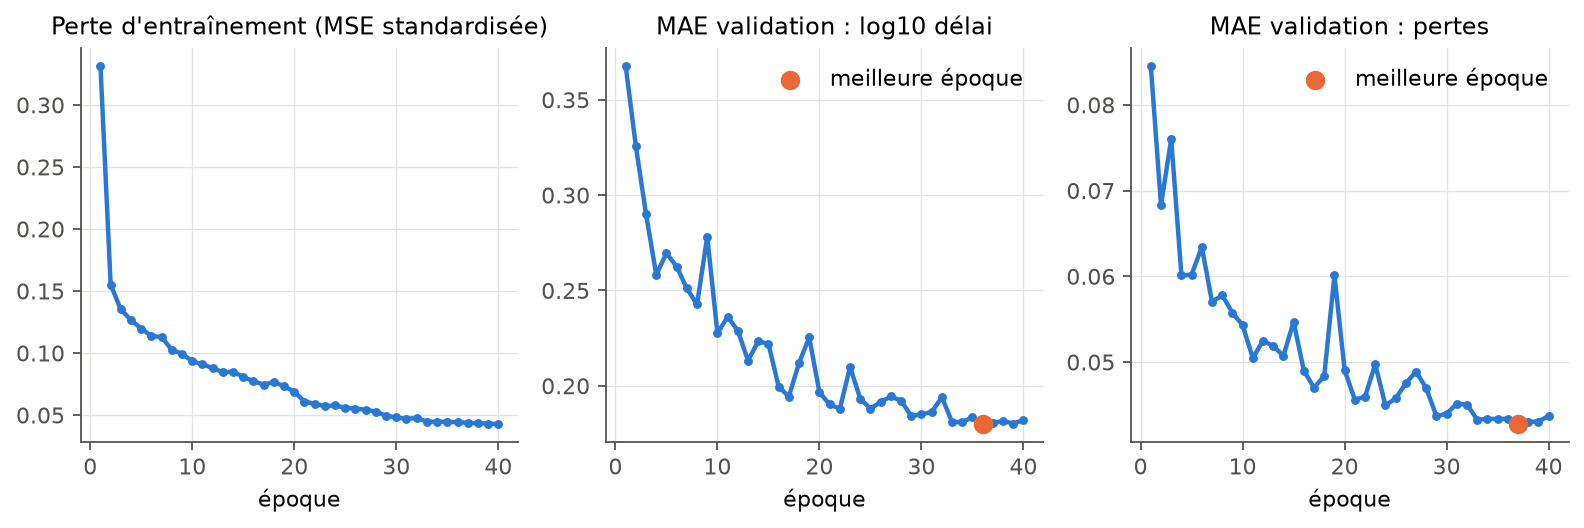
\includegraphics[width=\linewidth]{fig_training.png}
\caption{Courbes d'apprentissage du GNN : perte d'entraînement et MAE de validation (topologies inédites).}
\label{fig:training}
\end{figure}
La perte d'entraînement décroît régulièrement. La MAE de validation suit la même tendance, avec les oscillations attendues sur des topologies inédites, et atteint son minimum vers l'époque 36 (figure~\ref{fig:training}). On n'observe pas de divergence entre entraînement et validation, donc pas de surapprentissage marqué. La validation baisse encore légèrement à 40 époques : un entraînement plus long gagnerait probablement quelques centièmes. Trois initialisations donnent une MAE de test de 0,167 à 0,175 (écart-type de 0,004 décade).

\section{Comparaison globale et pendant les événements}
\begin{table}[H]
\centering\footnotesize
\adjustbox{max width=\linewidth}{\begin{tabular}{lrrrrrrr}
\toprule
Modèle & MAE global & MAE hors év. & MAE év. & MAE surch. & MAE délest. & MSE global & MSE év. \\
\midrule
Naïf & 0{,}825 & 0{,}686 & 1{,}707 & 1{,}723 & 1{,}644 & 1{,}286 & 4{,}612 \\
Ridge & 0{,}522 & 0{,}451 & 0{,}969 & 1{,}071 & 0{,}572 & 0{,}533 & 1{,}546 \\
Gradient Boosting & 0{,}276 & 0{,}215 & 0{,}664 & 0{,}749 & 0{,}335 & 0{,}311 & 1{,}130 \\
MLP & 0{,}343 & 0{,}286 & 0{,}705 & 0{,}797 & 0{,}344 & 0{,}362 & 1{,}211 \\
GNN & \textbf{0{,}175} & \textbf{0{,}159} & \textbf{0{,}271} & \textbf{0{,}312} & \textbf{0{,}111} & \textbf{0{,}140} & \textbf{0{,}255} \\
\bottomrule
\end{tabular}}
\caption{Cible log10(délai) : MAE et MSE (décades) sur le test, globalement et par sous-ensemble. En gras : le meilleur modèle.}
\label{tab:delai}
\end{table}
\begin{table}[H]
\centering\footnotesize
\adjustbox{max width=\linewidth}{\begin{tabular}{lrrrrrrr}
\toprule
Modèle & MAE global & MAE hors év. & MAE év. & MAE surch. & MAE délest. & MSE global & MSE év. \\
\midrule
Naïf & 0{,}196 & 0{,}153 & 0{,}472 & 0{,}549 & 0{,}173 & 0{,}089 & 0{,}314 \\
Ridge & 0{,}132 & 0{,}112 & 0{,}256 & 0{,}295 & 0{,}103 & 0{,}039 & 0{,}104 \\
Gradient Boosting & 0{,}067 & 0{,}053 & 0{,}154 & 0{,}186 & 0{,}028 & 0{,}020 & 0{,}066 \\
MLP & 0{,}082 & 0{,}067 & 0{,}173 & 0{,}207 & 0{,}041 & 0{,}023 & 0{,}076 \\
GNN & \textbf{0{,}045} & \textbf{0{,}039} & \textbf{0{,}078} & \textbf{0{,}095} & \textbf{0{,}010} & \textbf{0{,}010} & \textbf{0{,}024} \\
\bottomrule
\end{tabular}}
\caption{Cible taux de pertes : MAE et MSE sur le test.}
\label{tab:pertes}
\end{table}
\begin{figure}[H]
\centering
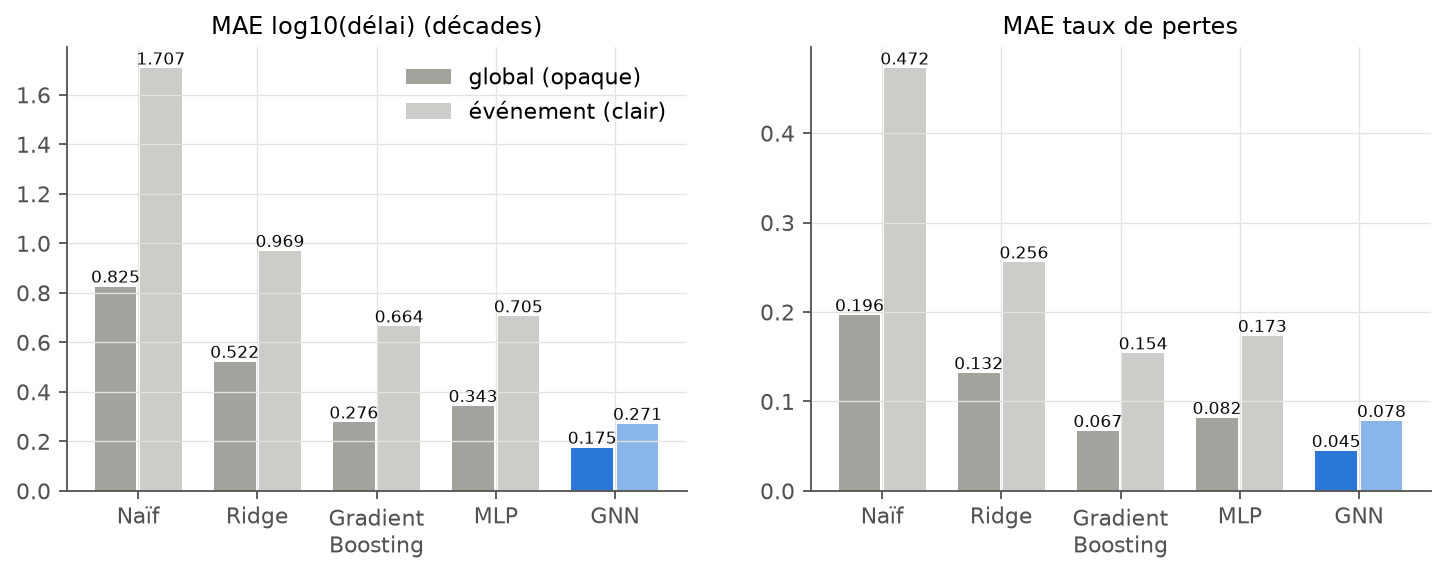
\includegraphics[width=\linewidth]{fig_comparison.png}
\caption{MAE globale (couleur pleine) et pendant les événements (couleur claire), pour les deux cibles.}
\label{fig:comparison}
\end{figure}

Les tableaux~\ref{tab:delai} et~\ref{tab:pertes} donnent un classement net et cohérent sur les deux cibles et les deux métriques.
\begin{itemize}
  \item \textbf{Naïf} (0,825 décade) et \textbf{Ridge} (0,522) restent loin derrière : la relation entre configuration et QoS est fortement non linéaire (coude en $b\approx1$).
  \item Le \textbf{Gradient Boosting} (0,276) est le meilleur modèle sans graphe, devant le \textbf{MLP} (0,343). Les deux voient exactement les mêmes 24 features.
  \item Le \textbf{GNN} réduit l'erreur de 37\,\% par rapport au Gradient Boosting (0,175) sur le délai, et de 33\,\% sur les pertes (0,045 contre 0,067). Sa MSE est 2,2 fois plus faible (0,140 contre 0,311) : il fait beaucoup moins de très grosses erreurs, ce que confirme la figure~\ref{fig:scatter}.
\end{itemize}

\paragraph{Pendant les événements.} Tous les modèles se dégradent, mais pas au même rythme.
\begin{itemize}
  \item La MAE du Gradient Boosting passe de 0,276 à 0,664 (×2,4), celle du MLP de 0,343 à 0,705, celle du GNN de 0,175 à 0,271 seulement (×1,55).
  \item En \textbf{surcharge}, le cas critique pour l'opérateur, le GNN se trompe de 0,31 décade, contre 0,75 pour le Gradient Boosting.
  \item En \textbf{délestage}, il reste au niveau du régime normal (0,11).
  \item Sur les pertes en événement, l'écart est d'un facteur 2 (0,078 contre 0,154).
\end{itemize}

\begin{figure}[H]
\centering
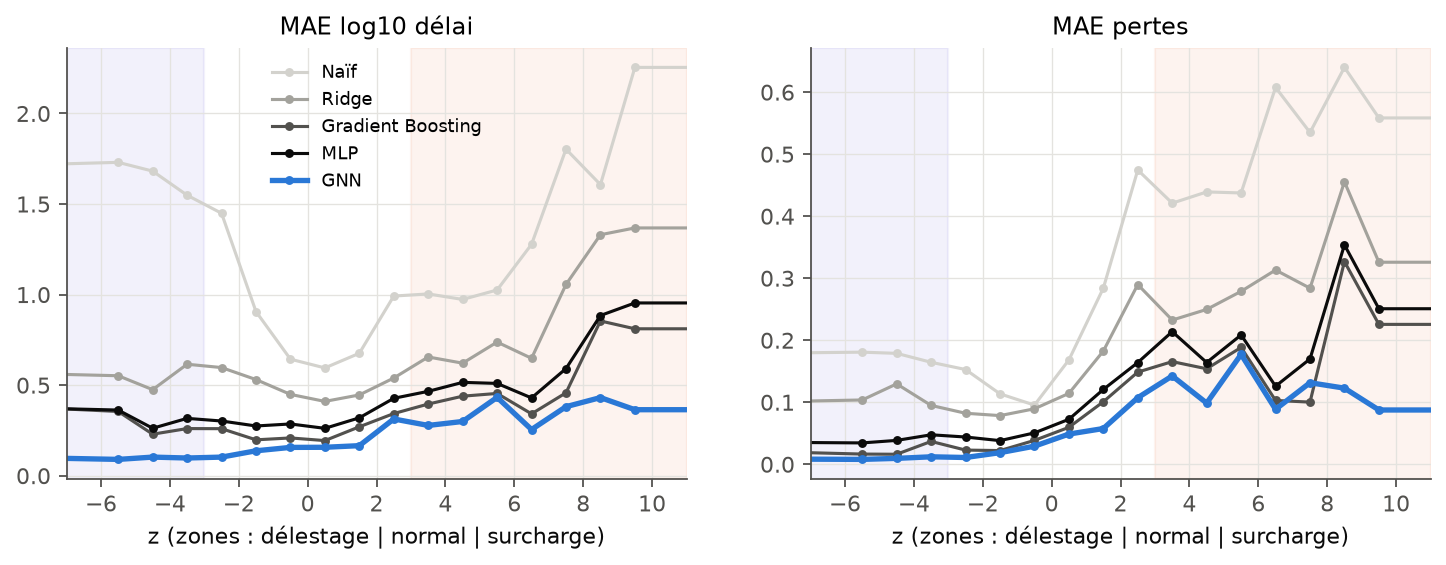
\includegraphics[width=\linewidth]{fig_errors_z.png}
\caption{MAE en fonction de l'écart $z$ au régime habituel (zones colorées : délestage à gauche, surcharge à droite).}
\label{fig:errors_z}
\end{figure}
La figure~\ref{fig:errors_z} montre la même chose en continu. Toutes les erreurs augmentent avec $z$ : plus la charge s'écarte du régime habituel, plus la prédiction est difficile, et l'hypothèse H2 est confirmée. C'est attendu : loin de la médiane, les configurations sont rares dans les données d'entraînement, et la QoS y est la plus sensible à la charge (zone de saturation, section~\ref{sec:sota-alloc}). La pente est cependant beaucoup plus faible pour le GNN. Côté délestage, son erreur ne bouge presque pas, alors que celle des modèles tabulaires remonte.

\begin{figure}[H]
\centering
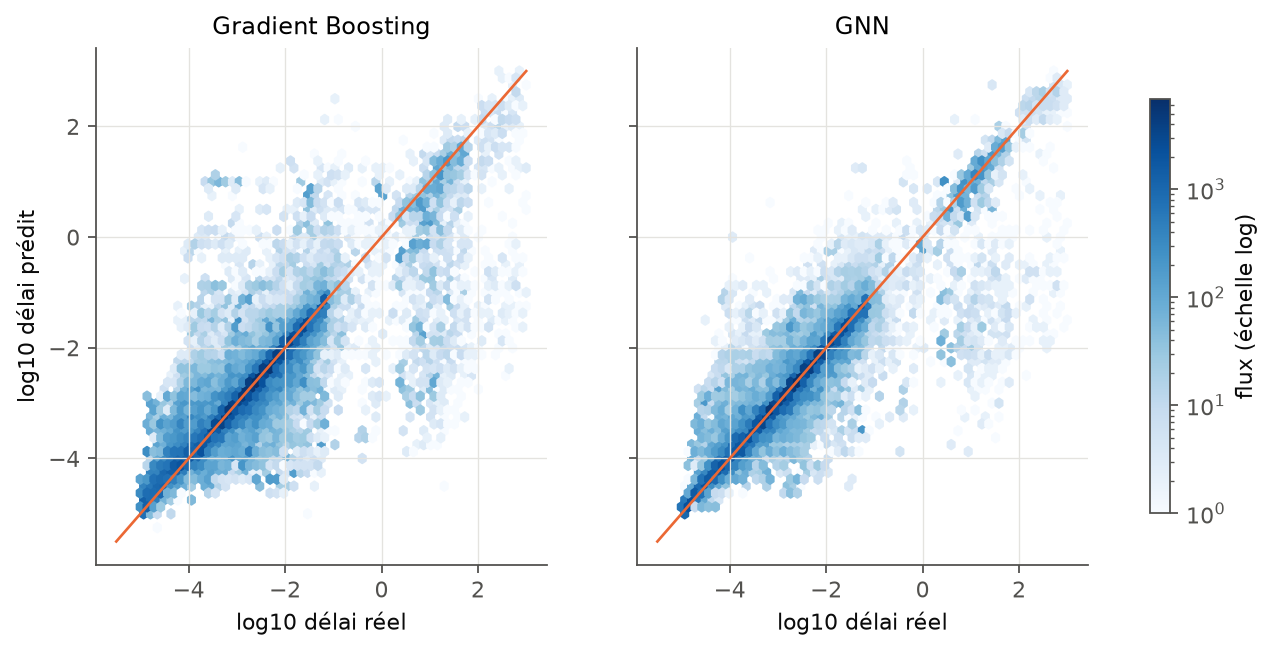
\includegraphics[width=0.85\linewidth]{fig_scatter.png}
\caption{Délai prédit contre délai réel (test, densité de flux en échelle log) : Gradient Boosting et GNN.}
\label{fig:scatter}
\end{figure}
Sur la figure~\ref{fig:scatter}, le nuage du Gradient Boosting présente des bandes horizontales et verticales : il confond les régimes congestionné et non congestionné. Le GNN se concentre beaucoup plus autour de la diagonale, y compris pour les délais extrêmes des files affamées (au-delà de 1~s).

\section{Par type de slice}
\begin{table}[H]
\centering\footnotesize
\adjustbox{max width=\linewidth}{\begin{tabular}{lrrrrrr}
\toprule
Modèle & MAE délai URLLC & MAE délai eMBB & MAE délai mMTC & MAE pertes URLLC & MAE pertes eMBB & MAE pertes mMTC \\
\midrule
Naïf & 0{,}753 & 0{,}654 & 0{,}857 & 0{,}217 & 0{,}208 & 0{,}190 \\
Ridge & 0{,}506 & 0{,}575 & 0{,}523 & 0{,}136 & 0{,}149 & 0{,}129 \\
Gradient Boosting & 0{,}246 & 0{,}340 & 0{,}282 & 0{,}058 & 0{,}092 & 0{,}068 \\
MLP & 0{,}305 & 0{,}382 & 0{,}352 & 0{,}070 & 0{,}105 & 0{,}083 \\
GNN & \textbf{0{,}194} & \textbf{0{,}257} & \textbf{0{,}164} & \textbf{0{,}047} & \textbf{0{,}071} & \textbf{0{,}042} \\
\bottomrule
\end{tabular}}
\caption{MAE par type de slice (test).}
\label{tab:slice}
\end{table}
Le classement est le même pour les trois slices (tableau~\ref{tab:slice}). eMBB est la plus difficile pour tous les modèles appris : peu de flux, de gros paquets, des files très sensibles à leur poids. C'est sur mMTC que le GNN gagne le plus : 0,164 contre 0,282. Les flux mMTC sont nombreux et petits, et leur QoS dépend surtout de la congestion créée par les autres slices sur les liens partagés.

\section{Utilité opérationnelle : détection des violations de SLA}
\begin{table}[H]
\centering\footnotesize
\adjustbox{max width=\linewidth}{\begin{tabular}{lrrrr}
\toprule
Modèle & Exact. équil. global & Exact. équil. événement & F1 violation global & F1 violation événement \\
\midrule
Naïf & 0{,}500 & 0{,}500 & 0{,}690 & 0{,}874 \\
Ridge & 0{,}765 & 0{,}746 & 0{,}778 & 0{,}905 \\
Gradient Boosting & 0{,}907 & 0{,}836 & 0{,}912 & 0{,}941 \\
MLP & 0{,}871 & 0{,}830 & 0{,}874 & 0{,}936 \\
GNN & \textbf{0{,}926} & \textbf{0{,}858} & \textbf{0{,}929} & \textbf{0{,}944} \\
\bottomrule
\end{tabular}}
\caption{Décision « délai prédit au-dessus du SLA ? » pour eMBB (10~ms) et URLLC (0,5~ms) : exactitude équilibrée et F1 de la classe « violation ».}
\label{tab:sla}
\end{table}
Transformée en décision binaire, la prédiction reste utile (tableau~\ref{tab:sla}). Le GNN atteint une exactitude équilibrée de 0,926 (0,858 pendant les événements), contre 0,907 (0,836) pour le Gradient Boosting et 0,500 pour le modèle naïf. L'écart est plus faible que sur la MAE : un flux loin du seuil est bien classé par tous les modèles non linéaires. Le gain du GNN porte surtout sur les flux proches du seuil et sur l'\emph{ampleur} des dégradations, qui compte pour choisir de combien augmenter une réservation.

\section{Ablation}
\begin{table}[H]
\centering\footnotesize
\adjustbox{max width=\linewidth}{\begin{tabular}{llrrrr}
\toprule
Modèle & Variante & MAE délai & Δ MAE délai & MAE pertes & Δ MAE pertes \\
\midrule
Ridge & complet & 0{,}522 & 0{,}000 & 0{,}132 & 0{,}000 \\
Ridge & sans réservation & 0{,}553 & 0{,}031 & 0{,}140 & 0{,}008 \\
Ridge & sans charge & 0{,}556 & 0{,}034 & 0{,}176 & 0{,}045 \\
Ridge & sans physique & 0{,}605 & 0{,}084 & 0{,}133 & 0{,}001 \\
Ridge & sans allocation & 0{,}605 & 0{,}083 & 0{,}154 & 0{,}022 \\
Gradient Boosting & complet & 0{,}276 & 0{,}000 & 0{,}067 & 0{,}000 \\
Gradient Boosting & sans réservation & 0{,}314 & 0{,}037 & 0{,}077 & 0{,}010 \\
Gradient Boosting & sans charge & 0{,}429 & 0{,}153 & 0{,}152 & 0{,}085 \\
Gradient Boosting & sans physique & 0{,}279 & 0{,}002 & 0{,}068 & 0{,}001 \\
Gradient Boosting & sans allocation & 0{,}453 & 0{,}176 & 0{,}128 & 0{,}061 \\
MLP & complet & 0{,}343 & 0{,}000 & 0{,}082 & 0{,}000 \\
MLP & sans réservation & 0{,}361 & 0{,}018 & 0{,}092 & 0{,}010 \\
MLP & sans charge & 0{,}448 & 0{,}105 & 0{,}154 & 0{,}073 \\
MLP & sans physique & 0{,}367 & 0{,}024 & 0{,}094 & 0{,}013 \\
MLP & sans allocation & 0{,}469 & 0{,}126 & 0{,}129 & 0{,}048 \\
GNN & complet & 0{,}175 & 0{,}000 & 0{,}045 & 0{,}000 \\
GNN & sans réservation & 0{,}179 & 0{,}004 & 0{,}046 & 0{,}001 \\
GNN & sans charge & 0{,}367 & 0{,}192 & 0{,}120 & 0{,}075 \\
GNN & sans physique & 0{,}182 & 0{,}008 & 0{,}043 & -0{,}002 \\
GNN & sans allocation & 0{,}402 & 0{,}227 & 0{,}114 & 0{,}069 \\
GNN & T = 0 (sans interactions) & 0{,}240 & 0{,}065 & 0{,}062 & 0{,}017 \\
GNN & sans nœuds file & 0{,}428 & 0{,}254 & 0{,}098 & 0{,}053 \\
\bottomrule
\end{tabular}}
\caption{Ablation (test) : MAE après retrait d'une famille de features, ou d'un élément de structure du GNN, et écart avec le modèle complet.}
\label{tab:ablation}
\end{table}
\begin{figure}[H]
\centering
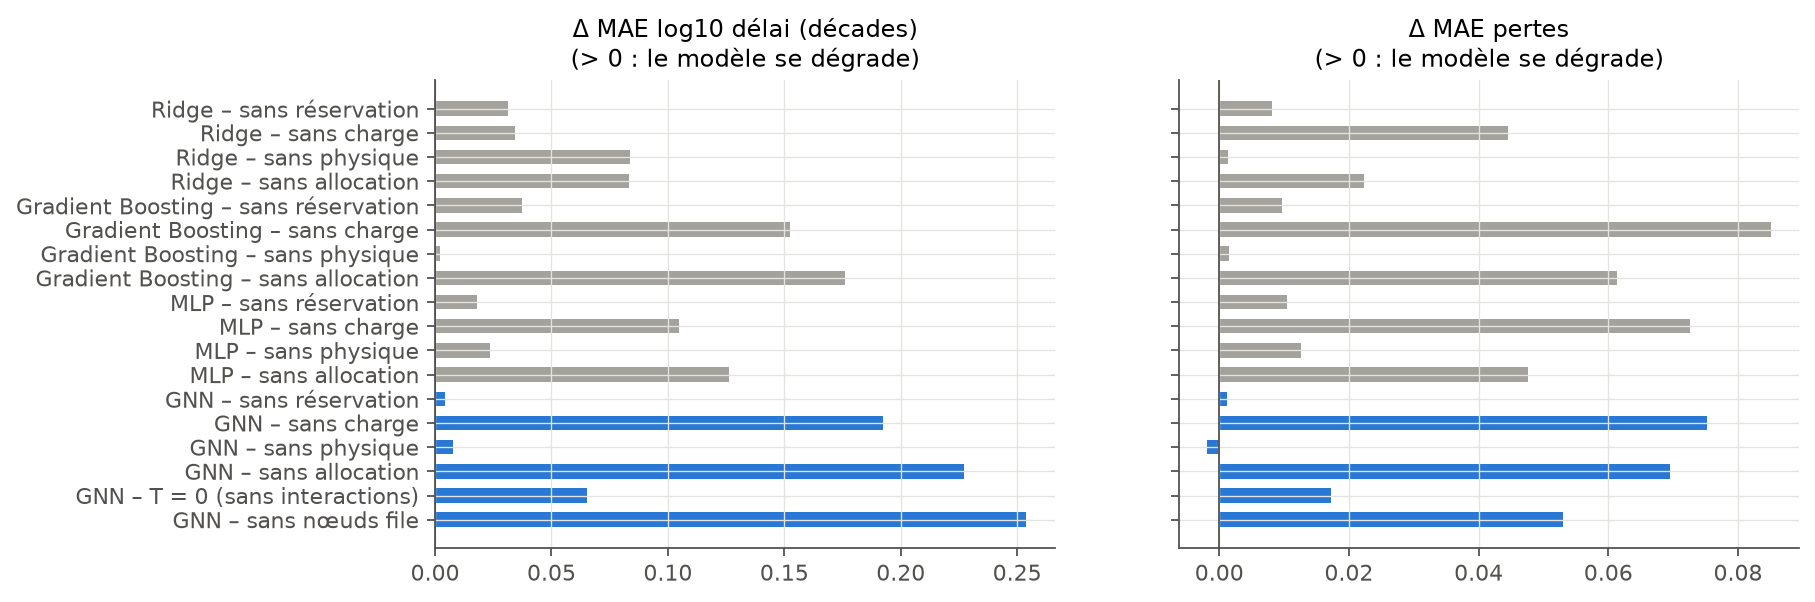
\includegraphics[width=\linewidth]{fig_ablation.png}
\caption{Hausse de la MAE après chaque ablation (en bleu : GNN).}
\label{fig:ablation}
\end{figure}
Le tableau~\ref{tab:ablation} et la figure~\ref{fig:ablation} répondent à trois questions.

\paragraph{D'où vient le gain du GNN ?}
\begin{itemize}
  \item Avec $T=0$, chaque flux ne lit qu'une fois l'état initial des liens et des files : pas de rétroaction, donc pas d'interaction entre flux. La MAE remonte alors à 0,240, et à 0,502 pendant les événements. Les interactions expliquent donc environ 60\,\% de l'écart avec le Gradient Boosting, globalement (0,065 sur 0,101 décade) comme pendant les événements (0,231 sur 0,393) : c'est l'hypothèse H1.
  \item Sans nœuds « file WFQ », le GNN tombe à 0,428, moins bon que le Gradient Boosting. La représentation explicite des réservations par slice est indispensable.
\end{itemize}

\paragraph{Quelles informations sont nécessaires ?} Retirer toute l'information d'\emph{allocation} ($\delta$, poids, débit réservé, délai de file pleine) fait passer le GNN de 0,175 à 0,402 (0,94 pendant les événements) et le Gradient Boosting de 0,276 à 0,453. Retirer la \emph{charge} coûte presque autant : 0,367 pour le GNN. Les deux familles sont nécessaires, ce qui confirme l'hypothèse H3. Les familles « réservation » et « physique » sont en revanche redondantes : le délai de file pleine dépend du débit WFQ effectif, donc du poids. Retirer l'une sans l'autre ne coûte presque rien, d'où la variante « allocation » qui retire les deux.

\paragraph{La connaissance du domaine aide-t-elle ?} La feature physique (délai de file pleine) est la plus importante pour le Gradient Boosting (figure~\ref{fig:importance}). Elle améliore nettement Ridge : 0,605 sans elle, 0,522 avec. Elle n'apporte presque rien au GNN (0,182 sans, 0,175 avec), qui reconstruit cette relation à partir des poids, des capacités et des tailles de paquets.

\begin{figure}[H]
\centering
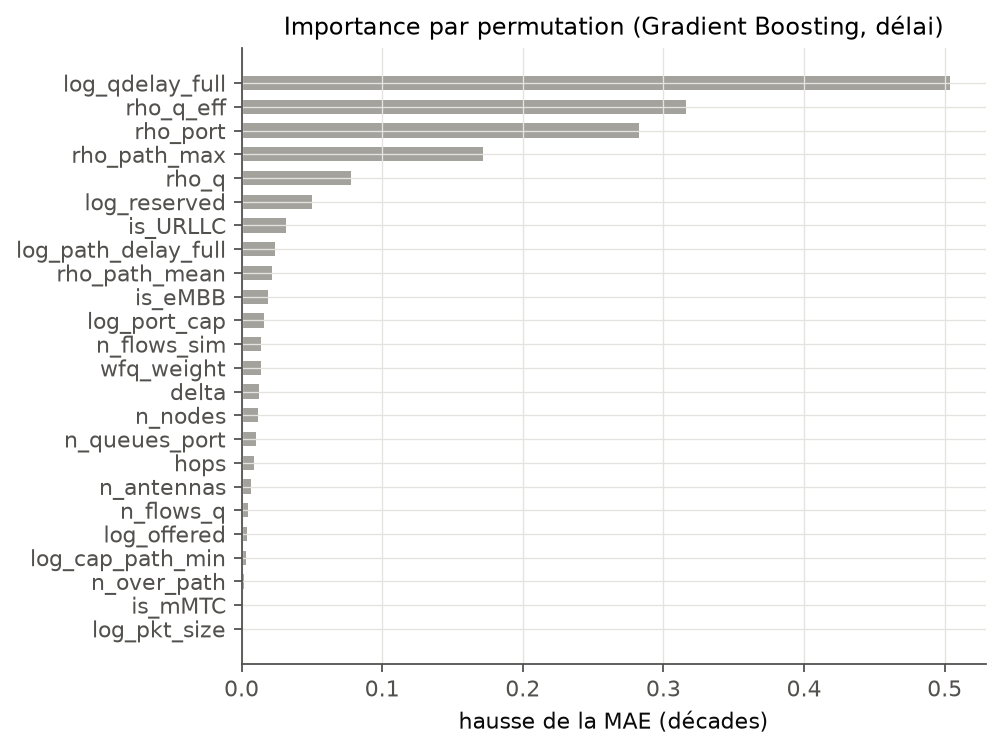
\includegraphics[width=0.62\linewidth]{fig_importance.png}
\caption{Importance par permutation~\cite{breiman} des features du Gradient Boosting (cible délai, test) : hausse de la MAE quand on mélange une feature.}
\label{fig:importance}
\end{figure}

\section{Décalage de distribution : grands réseaux}
\begin{table}[H]
\centering\footnotesize
\adjustbox{max width=\linewidth}{\begin{tabular}{lrrrrr}
\toprule
Modèle & MAE délai (topo) & MAE délai (grands) & MAE pertes (topo) & MAE pertes (grands) & MAE délai (grands, év.) \\
\midrule
Naïf & 0{,}825 & 0{,}840 & 0{,}196 & 0{,}206 & 1{,}556 \\
Ridge & 0{,}522 & 0{,}552 & 0{,}132 & 0{,}139 & 0{,}837 \\
Gradient Boosting & 0{,}276 & 0{,}293 & 0{,}067 & 0{,}075 & 0{,}573 \\
MLP & 0{,}343 & 0{,}361 & 0{,}082 & 0{,}091 & 0{,}600 \\
GNN & \textbf{0{,}175} & \textbf{0{,}203} & \textbf{0{,}045} & \textbf{0{,}053} & \textbf{0{,}283} \\
\bottomrule
\end{tabular}}
\caption{MAE sur le test du découpage aléatoire (« topo ») et sur le test des grands réseaux (« grands », topologies de 212 nœuds et plus, absentes de l'entraînement).}
\label{tab:shift}
\end{table}
\begin{figure}[H]
\centering
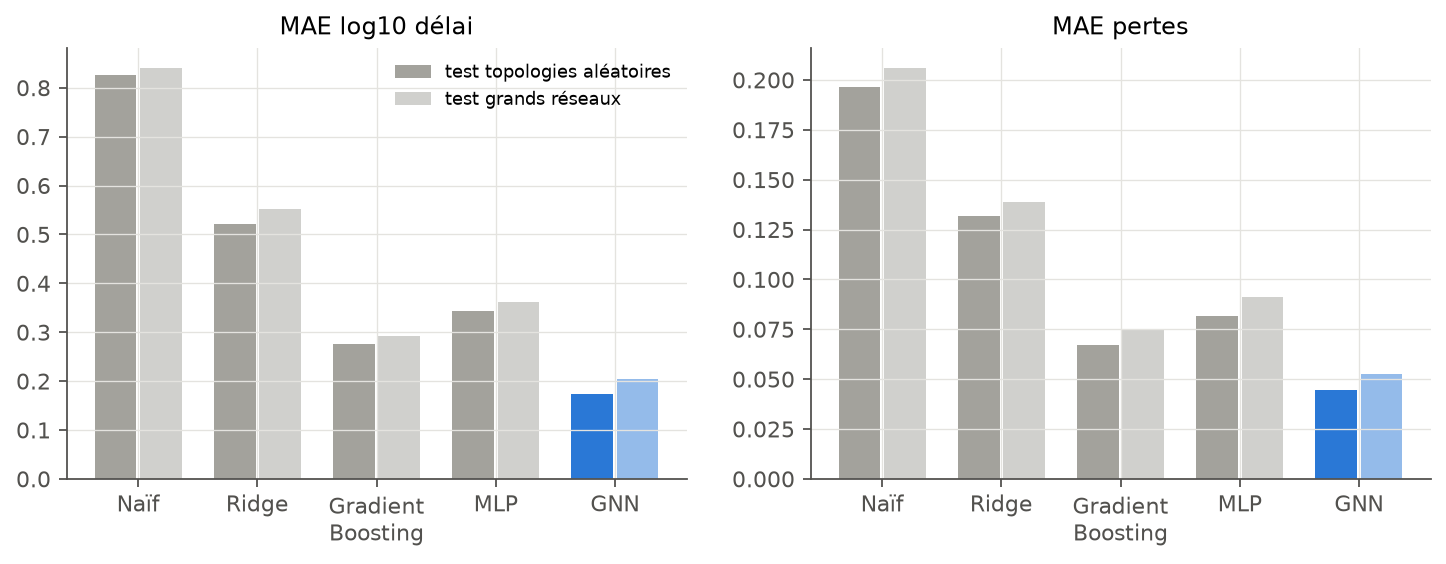
\includegraphics[width=\linewidth]{fig_shift.png}
\caption{Effet du décalage de distribution sur la taille des réseaux.}
\label{fig:shift}
\end{figure}
Entraînés sur les petits et moyens réseaux puis testés sur les plus grands, tous les modèles se dégradent un peu (tableau~\ref{tab:shift}). C'est un décalage de covariables~\cite{datasetshift} : la loi des entrées change (chemins plus longs, liens plus partagés), pas la physique qui relie entrées et QoS.
\begin{itemize}
  \item Le GNN passe de 0,175 à 0,203 (+16\,\%), le Gradient Boosting de 0,276 à 0,293 (+6\,\%).
  \item Le GNN reste nettement le meilleur, y compris pendant les événements de ces grands réseaux : 0,283 contre 0,573.
  \item Sa dégradation relative plus forte rappelle qu'un GNN généralise à des tailles nouvelles sans garantie : les chemins plus longs et les liens plus partagés sortent de ce qu'il a vu. Il n'a en revanche besoin d'aucune adaptation pour s'appliquer à un graphe plus grand.
\end{itemize}

%=====================================================================
\chapter{Discussion}\label{chap:disc}
%=====================================================================
\section{Réponses aux questions d'analyse du guide}
\begin{description}
  \item[Quel modèle généralise le mieux ?] Le GNN, sur des topologies jamais vues (MAE de 0,175 décade sur le délai et de 0,045 sur les pertes) comme sur des réseaux plus grands que ceux de l'entraînement (0,203). L'écart avec le Gradient Boosting est environ 25 fois plus grand que la variabilité due à l'initialisation.
  \item[Quel modèle résiste le mieux aux événements ?] Le GNN : son erreur n'augmente que de 55\,\% pendant les événements, contre 140\,\% pour le Gradient Boosting. En surcharge, il est 2,4 fois plus précis.
  \item[Le GNN apporte-t-il un gain réel ?] Oui : $-37\,\%$ de MAE globalement et $-59\,\%$ pendant les événements, avec une cause identifiée par l'ablation (interactions entre flux et files WFQ explicites). En décision SLA binaire, le gain est réel mais plus modeste (+0,02 d'exactitude équilibrée).
  \item[Quelles features sont importantes ?] L'allocation (poids WFQ et grandeurs qui en dérivent) et la charge des files, du port et des liens. La structure de la topologie seule et le type de slice comptent peu. Pour les modèles sans graphe, le délai de file pleine, une connaissance du domaine, est la feature dominante.
  \item[Les performances changent-elles quand la distribution diffère ?] Oui, modérément : de +2 à +16\,\% d'erreur sur les grands réseaux selon le modèle, sans changement de classement.
  \item[Quelles sont les limites ?] Voir la section~\ref{sec:limites}.
\end{description}

\section{« Meilleur score » ne veut pas dire « meilleure solution »}
Le GNN a le meilleur score, mais son coût est plus élevé. Il faut environ 16~minutes d'entraînement sur GPU (cinq fois plus sur CPU), contre 2~minutes pour le Gradient Boosting. Il demande aussi de construire un graphe par configuration et il est plus difficile à expliquer. Pour un contrôle d'admission grossier, loin des seuils, un Gradient Boosting bien alimenté en features physiques donne déjà 0,907 d'exactitude équilibrée. Le GNN se justifie quand on a besoin de l'\emph{ampleur} des dégradations et d'une fiabilité dans les situations inhabituelles, c'est-à-dire pour la gestion \emph{dynamique} des slices.

\section{Trois choix méthodologiques défendus}
\begin{enumerate}
  \item \textbf{Vérifier les entrées contre les sorties avant de modéliser.} Confronter la charge offerte calculée à l'utilisation mesurée a révélé que 42\,\% des chemins du fichier de slices étaient faux. Sans cette vérification, tous les modèles auraient appris sur des entrées erronées, sans aucun message d'erreur. La qualité des données a ici pesé plus lourd que le choix du modèle.
  \item \textbf{Découper par topologie et évaluer par flux.} Le découpage par topologie empêche de mémoriser un réseau. Les classes de flux pondérées rendent le calcul six fois plus léger sans changer une seule métrique.
  \item \textbf{Définir les événements sur les entrées, en log, avec une règle robuste.} Le masque est observable par l'opérateur avant toute mesure, il ne dépend pas de la cible (pas de biais de sélection) et il est cohérent avec la physique du problème : coude en $b\approx1$, écarts multiplicatifs, queues lourdes d'où la règle de Hampel.
\end{enumerate}

\section{Limites}\label{sec:limites}
\begin{itemize}
  \item \textbf{Un seul simulateur}, des régimes stationnaires et un réseau de transport filaire sans partie radio : les conclusions valent pour ce cadre.
  \item \textbf{Événements reconstruits} : faute d'axe temporel, un événement est un écart au régime habituel de la topologie, pas une transition observée. Le comportement \emph{pendant} la transition (régime transitoire) n'est pas étudié.
  \item \textbf{Défauts du dataset} : une partie des surcharges vient des réservations hors chemin. Elles sont réelles dans les simulations, mais un opérateur ne les produirait probablement pas volontairement.
  \item \textbf{Variabilité} estimée seulement sur l'initialisation du GNN (3 graines), pas sur la découpe des topologies ; hyperparamètres du GNN non optimisés ; entraînement arrêté à 40 époques alors que la validation baissait encore légèrement.
  \item \textbf{Prédiction et non décision} : le modèle évalue une allocation, il ne choisit pas $\delta$. Une boucle d'optimisation (recherche des poids minimaux respectant les SLA) reste à construire.
\end{itemize}

%=====================================================================
\chapter{Conclusion}\label{chap:concl}
%=====================================================================
Nous avons construit un jumeau numérique de la QoS des slices à partir du dataset \emph{B5G Network Slicing}. Il prédit le délai et les pertes de chaque flux à partir de la configuration du réseau et des réservations WFQ. Après correction de plusieurs défauts du dataset, un GNN hétérogène flux / files WFQ / liens prédit le délai avec une erreur typique d'un facteur 1,5. Il réduit l'erreur de 37\,\% par rapport au meilleur modèle sans graphe, et de 59\,\% pendant les changements brusques du réseau, là où les modèles tabulaires se dégradent le plus.

\paragraph{Réponse à la question finale.} \emph{Dans quelles conditions une approche GNN apporte-t-elle une valeur ajoutée pour la gestion dynamique des slices B5G ?} Nos expériences en identifient quatre :
\begin{enumerate}
  \item \textbf{quand la QoS dépend de ressources partagées et d'effets en cascade} (congestion des liens communs, pertes en amont) que des features par flux ne peuvent pas résumer. L'ablation $T=0$ montre que la rétroaction flux $\leftrightarrow$ liens est la source principale du gain ;
  \item \textbf{quand le graphe représente explicitement le levier de gestion}, ici les files WFQ par slice. Un GNN qui ne les voit pas perd tout son avantage ;
  \item \textbf{quand le réseau sort de son régime habituel} (surcharges, délestages). C'est le cas d'usage de la gestion dynamique, et c'est là que l'écart avec les modèles tabulaires est le plus grand ;
  \item \textbf{quand la topologie change ou grandit} : le même modèle s'applique à des réseaux inédits, avec une dégradation modérée.
\end{enumerate}
À l'inverse, pour des décisions grossières loin des seuils, ou quand le coût d'entraînement compte, un Gradient Boosting nourri de features physiques reste une alternative solide. L'étape suivante consiste à boucler le jumeau numérique avec un optimiseur des réservations $\delta$, et à le valider sur des traces temporelles réelles.


\appendix
%=====================================================================
\chapter{Reproduction}\label{chap:annexe}
%=====================================================================
\begin{table}[H]
\centering\small
\begin{tabularx}{\linewidth}{@{}lX@{}}
\toprule
Fichier & Rôle\\
\midrule
\texttt{projet\_B5G\_slicing\_GNN.ipynb} & notebook complet : EDA, protocole, modèles, événements, GNN, comparaison\\
\texttt{code/extraction.py} & lecture des archives brutes $\to$ 4 tables Parquet (environ 6~min sur 14 processus)\\
\texttt{code/features.py} & 24 features par flux à partir des entrées ; regroupement en classes de flux\\
\texttt{code/preparation.py} & classes de flux, masque d'événements, graphes (environ 3~min)\\
\texttt{code/splits.py} & découpages par topologie (\texttt{topo}, \texttt{shift})\\
\texttt{code/run\_tabular.py} & modèle naïf, Ridge, Gradient Boosting, MLP\\
\texttt{code/gnn.py}, \texttt{code/run\_gnn.py} & SliceGNN et son entraînement (CPU ou GPU)\\
\texttt{code/evaluation.py} & MAE et MSE pondérées par flux\\
\path{Guide_du_code.pdf} & guide détaillé de chaque fichier du code et aide-mémoire « où est… ? »\\
\texttt{presentation/} & présentation, script de génération et discours minuté\\
\bottomrule
\end{tabularx}
\caption{Organisation du code.}
\end{table}
Ordre d'exécution :
\begin{enumerate}[nosep]
  \item télécharger le dataset Zenodo dans \texttt{data/raw/} et le décompresser ;
  \item lancer \texttt{bash code/run\_all.sh} (extraction, préparation, tous les entraînements) ;
  \item exécuter le notebook, qui relit les résultats en cache dans \texttt{results/} et relance les entraînements manquants.
\end{enumerate}

\begin{thebibliography}{99}\addcontentsline{toc}{chapter}{\bibname}\small
\bibitem{farreras} M.~Farreras, J.~Paillissé, L.~Fàbrega, P.~Vilà. Generation of a network slicing dataset: The foundations for AI-based B5G resource management. \emph{Data in Brief}, 55, 110738, 2024. Données : \url{https://doi.org/10.5281/zenodo.10610616}.
\bibitem{routenet} K.~Rusek, J.~Suárez-Varela, P.~Almasan, P.~Barlet-Ros, A.~Cabellos-Aparicio. RouteNet: Leveraging Graph Neural Networks for network modeling and optimization in SDN. \emph{IEEE JSAC}, 38(10), 2020.
\bibitem{routenetf} M.~Ferriol-Galmés, J.~Paillissé, J.~Suárez-Varela, K.~Rusek, S.~Xiao, X.~Shi, X.~Cheng, P.~Barlet-Ros, A.~Cabellos-Aparicio. RouteNet-Fermi: Network Modeling with Graph Neural Networks. \emph{IEEE/ACM Transactions on Networking}, 2023.
\bibitem{gcn} T.~N.~Kipf, M.~Welling. Semi-Supervised Classification with Graph Convolutional Networks. \emph{ICLR}, 2017.
\bibitem{sage} W.~Hamilton, R.~Ying, J.~Leskovec. Inductive Representation Learning on Large Graphs. \emph{NeurIPS}, 2017.
\bibitem{gat} P.~Veličković, G.~Cucurull, A.~Casanova, A.~Romero, P.~Liò, Y.~Bengio. Graph Attention Networks. \emph{ICLR}, 2018.
\bibitem{gru} K.~Cho et al. Learning Phrase Representations using RNN Encoder--Decoder for Statistical Machine Translation. \emph{EMNLP}, 2014.
\bibitem{wfq} A.~Demers, S.~Keshav, S.~Shenker. Analysis and simulation of a fair queueing algorithm. \emph{ACM SIGCOMM}, 1989.
\bibitem{itu2083} ITU-R. Recommendation M.2083-0 : IMT Vision -- Framework and overall objectives of the future development of IMT for 2020 and beyond. 2015.
\bibitem{tr38913} 3GPP. TR 38.913 : Study on scenarios and requirements for next generation access technologies.
\bibitem{ts23501} 3GPP. TS 23.501 : System architecture for the 5G System (5GS).
\bibitem{ts28530} 3GPP. TS 28.530 : Management and orchestration ; Concepts, use cases and requirements.
\bibitem{ngmn} NGMN Alliance. 5G White Paper. 2015.
\bibitem{foukas} X.~Foukas, G.~Patounas, A.~Elmokashfi, M.~K.~Marina. Network Slicing in 5G: Survey and Challenges. \emph{IEEE Communications Magazine}, 55(5), 2017.
\bibitem{afolabi} I.~Afolabi, T.~Taleb, K.~Samdanis, A.~Ksentini, H.~Flinck. Network Slicing and Softwarization: A Survey on Principles, Enabling Technologies, and Solutions. \emph{IEEE Communications Surveys \& Tutorials}, 20(3), 2018.
\bibitem{rost} P.~Rost et al. Network Slicing to Enable Scalability and Flexibility in 5G Mobile Networks. \emph{IEEE Communications Magazine}, 55(5), 2017.
\bibitem{gps} A.~K.~Parekh, R.~G.~Gallager. A generalized processor sharing approach to flow control in integrated services networks: the single-node case. \emph{IEEE/ACM Transactions on Networking}, 1(3), 1993.
\bibitem{kleinrock} L.~Kleinrock. \emph{Queueing Systems, Volume 1: Theory}. Wiley, 1975.
\bibitem{omnet} A.~Varga, R.~Hornig. An overview of the OMNeT++ simulation environment. \emph{SIMUTools}, 2008.
\bibitem{topozoo} S.~Knight, H.~X.~Nguyen, N.~Falkner, R.~Bowden, M.~Roughan. The Internet Topology Zoo. \emph{IEEE JSAC}, 29(9), 2011.
\bibitem{deepcog} D.~Bega, M.~Gramaglia, M.~Fiore, A.~Banchs, X.~Costa-Pérez. DeepCog: Cognitive Network Management in Sliced 5G Networks with Deep Learning. \emph{IEEE INFOCOM}, 2019.
\bibitem{digitaltwin} P.~Almasan et al. Network Digital Twin: Context, Enabling Technologies, and Opportunities. \emph{IEEE Communications Magazine}, 60(11), 2022.
\bibitem{battaglia} P.~W.~Battaglia et al. Relational inductive biases, deep learning, and graph networks. \emph{arXiv:1806.01261}, 2018.
\bibitem{mpnn} J.~Gilmer, S.~S.~Schoenholz, P.~F.~Riley, O.~Vinyals, G.~E.~Dahl. Neural Message Passing for Quantum Chemistry. \emph{ICML}, 2017.
\bibitem{gatv2} S.~Brody, U.~Alon, E.~Yahav. How Attentive are Graph Attention Networks? \emph{ICLR}, 2022.
\bibitem{gin} K.~Xu, W.~Hu, J.~Leskovec, S.~Jegelka. How Powerful are Graph Neural Networks? \emph{ICLR}, 2019.
\bibitem{ggnn} Y.~Li, D.~Tarlow, M.~Brockschmidt, R.~Zemel. Gated Graph Sequence Neural Networks. \emph{ICLR}, 2016.
\bibitem{rgcn} M.~Schlichtkrull, T.~N.~Kipf, P.~Bloem, R.~van den Berg, I.~Titov, M.~Welling. Modeling Relational Data with Graph Convolutional Networks. \emph{ESWC}, 2018.
\bibitem{han} X.~Wang et al. Heterogeneous Graph Attention Network. \emph{The Web Conference (WWW)}, 2019.
\bibitem{oversmoothing} Q.~Li, Z.~Han, X.-M.~Wu. Deeper Insights into Graph Convolutional Networks for Semi-Supervised Learning. \emph{AAAI}, 2018.
\bibitem{oversquashing} U.~Alon, E.~Yahav. On the Bottleneck of Graph Neural Networks and its Practical Implications. \emph{ICLR}, 2021.
\bibitem{suarez} J.~Suárez-Varela et al. Graph Neural Networks for Communication Networks: Context, Use Cases and Opportunities. \emph{IEEE Network}, 37(3), 2023.
\bibitem{jiang} W.~Jiang. Graph-based deep learning for communication networks: A survey. \emph{Computer Communications}, 185, 2022.
\bibitem{eisen} M.~Eisen, A.~Ribeiro. Optimal Wireless Resource Allocation With Random Edge Graph Neural Networks. \emph{IEEE Transactions on Signal Processing}, 68, 2020.
\bibitem{shen} Y.~Shen, Y.~Shi, J.~Zhang, K.~B.~Letaief. Graph Neural Networks for Scalable Radio Resource Management: Architecture Design and Theoretical Analysis. \emph{IEEE JSAC}, 39(1), 2021.
\bibitem{tofallis} C.~Tofallis. A better measure of relative prediction accuracy for model selection and model estimation. \emph{Journal of the Operational Research Society}, 66(8), 2015.
\bibitem{roberts} D.~R.~Roberts et al. Cross-validation strategies for data with temporal, spatial, hierarchical, or phylogenetic structure. \emph{Ecography}, 40(8), 2017.
\bibitem{kaufman} S.~Kaufman, S.~Rosset, C.~Perlich, O.~Stitelman. Leakage in data mining: Formulation, detection, and avoidance. \emph{ACM Transactions on Knowledge Discovery from Data}, 6(4), 2012.
\bibitem{ridge} A.~E.~Hoerl, R.~W.~Kennard. Ridge Regression: Biased Estimation for Nonorthogonal Problems. \emph{Technometrics}, 12(1), 1970.
\bibitem{friedman} J.~H.~Friedman. Greedy function approximation: A gradient boosting machine. \emph{Annals of Statistics}, 29(5), 2001.
\bibitem{lightgbm} G.~Ke et al. LightGBM: A Highly Efficient Gradient Boosting Decision Tree. \emph{NeurIPS}, 2017.
\bibitem{adam} D.~P.~Kingma, J.~Ba. Adam: A Method for Stochastic Optimization. \emph{ICLR}, 2015.
\bibitem{prechelt} L.~Prechelt. Early Stopping -- But When? In \emph{Neural Networks: Tricks of the Trade}, Springer, 1998.
\bibitem{breiman} L.~Breiman. Random Forests. \emph{Machine Learning}, 45, 2001.
\bibitem{datasetshift} J.~Quiñonero-Candela, M.~Sugiyama, A.~Schwaighofer, N.~D.~Lawrence (éd.). \emph{Dataset Shift in Machine Learning}. MIT Press, 2009.
\bibitem{hampel} F.~R.~Hampel. The Influence Curve and its Role in Robust Estimation. \emph{Journal of the American Statistical Association}, 69(346), 1974.
\bibitem{leys} C.~Leys, C.~Ley, O.~Klein, P.~Bernard, L.~Licata. Detecting outliers: Do not use standard deviation around the mean, use absolute deviation around the median. \emph{Journal of Experimental Social Psychology}, 49(4), 2013.
\bibitem{mad} P.~J.~Rousseeuw, C.~Croux. Alternatives to the Median Absolute Deviation. \emph{Journal of the American Statistical Association}, 88(424), 1993.
\end{thebibliography}

\end{document}
